\documentclass[12pt]{report} % 12 pt front size
\usepackage[a4 paper, top=25mm, bottom=25mm]{geometry} % page dimensions
\headheight= 15pt
\usepackage[utf8]{inputenc} %font used is Times new roman which is the standard font for articles

%Bibliography package
\usepackage[backend=biber,style=nature]{biblatex}
% .bib is the name of the file which contains the list of references for citation
\addbibresource{references.bib}
\usepackage{fancyhdr} %for header and footer
\pagestyle{fancy}
\fancyhf{}
\usepackage{float}
\usepackage{subcaption}
\usepackage{color}
\usepackage{setspace}
\setstretch{1.5} %linespacing can be changed as per requirement
\usepackage{import}
\usepackage{titlesec}
\usepackage[export]{adjustbox}
\usepackage{tocloft}
\usepackage{supertabular}
\renewcommand\cftchapaftersnum{.}
\renewcommand\cftsecaftersnum{.}
\renewcommand\thechapter{\Roman{chapter}}
\renewcommand\thesection{\arabic{section}}
\setcounter{secnumdepth}{3} %shows detailed contents with higher sub divisions (3)
\setcounter{tocdepth}{3}
\usepackage{amsmath}
\usepackage{graphicx} %allows the user to use the graphics env
\graphicspath{{./Images/}} % The folder where the images will be uploaded
\usepackage{caption} %Allows the user to use the caption in tables and figures
\usepackage[labelfont=bf]{caption}
\captionsetup[figure]{labelsep=space,singlelinecheck=off}
\usepackage[normalem]{ulem}
\useunder{\uline}{\ul}{}
\tolerance=1
\emergencystretch=\maxdimen
\hyphenpenalty=10000
\hbadness=10000
\fancyhead[R]{20th Nov. 2023}
\fancyhead[L]{Department of Mechanical Engineering, UCL}
\fancyfoot[R]{\thepage}
\renewcommand{\headrulewidth}{2pt} % the horizontal line at the top of the page
\renewcommand{\footrulewidth}{1pt} % the horizontal line at the bottom of the page

\begin{document} % beginning of the document
% ==================== Start of Cover Page ==================== %
\begin{titlepage}
\begin{center}
        \begin{center}
        
\includegraphics[width=.70\textwidth]{Image/ucl_logo.png}
        \vspace{0.5cm}
        \end{center}
        \vspace*{0.1cm}
        % Title
        \vspace{2cm}
        {\LARGE\textbf{MECH0064 MSc Group Design Project\\}}

        % Sub-Title
        \vspace{2cm}
        {\Huge\textbf{Compact Continuum Robotic\\}}
        \vspace{0.25cm}
        {\Huge\textbf{Manipulator Platform\\}}

        \vfill

        \begin{flushleft}
        \textbf{\emph{Group members:}} \\
        Zehao Ye (23119333)~~ Yuhao Zhu (23041703)\\ 
        Zehao Ye (23119333)~~ Zehao Ye (23119333)\\ 
        Zehao Ye (23119333)~~ Zehao Ye (23119333)\\ 
        \textbf{\emph{Supervised by} Dr Reza Haqshenas}
        \end{flushleft}
        \vspace{0.8cm}
\end{center}
\end{titlepage}
% ==================== End of Cover Page ==================== %

 % Cover Page
%%%%% Abstract %%%%%
\section*{Abstract} 
This is the Abstract of the final report. \\
AAAAA


\vfill


\textbf{\emph{Key Words: Continuum Robotic e.g.}}
\vspace{0.8cm}
\pagenumbering{gobble}
\setcounter{page}{1}
\newpage % Abstract
% contents
\tableofcontents
\addtocontents{toc}{~\hfill\textbf{Page}\par}
\begin{flushleft}
\phantomsection\addcontentsline{toc}{section}{Abstract}
\end{flushleft}

\setcounter{page}{1}
\newpage 
% list of figure
\listoffigures
\addcontentsline{toc}{chapter}{List of Figures}
\newpage
% list of table
\listoftables 
\addcontentsline{toc}{chapter}{List of Tables} 
\newpage
 % Contents, List of Figures, and List of Tables
%%%%% Introduction %%%%%
\section{Introduction} 
\subsection{Background}
This is the background part.
\subsection{Motivation}
This is the motivation part.

\subsection{Introduction}
Continuum robots has emerged and attracted a lot of attention since 2008 \cite{review_2008}. Before that, rigid 
joint robots were dominating the robotic arm industry. Compared with traditional rigid joint manipulator, continuum 
robots stand out for their flexible, highly bendable structure and extremely flexible motion performance. The 
limitations of rigid joint robots have gradually shown up in applications requiring highly detailed operation and 
in complex or space-limited environments. Thus, the continuum robot was developed and perfected during the years. 
This new kind of robot not only changes the code of traditional robot design but also demonstrates unprecedented 
application potential in fields such as exploration industry and medical science \cite{CR_medical_application}. 
Meanwhile, rigid-flexible-soft coupled continuum robots combine the multiple advantages of the stability of rigid 
structures, the flexibility of bendable structures, and the compliance of soft structures, and are one of the most 
promising robots for increasingly complex tasks \cite{fishboneCR}. \\
With unique bionic structure and motion characteristics, continuum robots provide new possibilities to solve these 
challenges. \\
This paper will discuss different types of existing continuum robots and their working principles, advantages, 
and disadvantages, then propose a proper continuum robot design that can be mainly applied to medical applications.

% change to new page
\newpage % Introduction
%%%%% Literature Review %%%%%
\section{Literature Review} 
In the last two decades, significant progress in electronic and computer technologies has led to remarkable 
growth in the field of manipulator robotics. Manipulators developed by various institutions have been integrated 
into the industrial sector to autonomously or semi-autonomously perform repetitive tasks. Simultaneously, 
manipulators are utilized for tasks with stringent precision requirements to minimize errors. Additionally, 
essential tasks are undertook by manipulators to substitute for humans in challenging environments. 
\subsection{Manipulators in Biology Field}
With a growing emphasis on the field of biology, manipulators have also been introduced to provide assistance. 
In the field of medicine, manipulators have been utilized since the end of the last century. The AESOP robotic 
surgical system, proposed by Computer Motion founded by Yulun Wang in 1993, was investigated in laparoscopic 
surgery in 1997 \cite{AESOP}. Afterward, the ZEUS robotic surgical system endowed with a trilateral manipulator 
configuration was proposed by Computer Motion in 1998 \cite{ZEUS}.During the period from 1999 to 2001, the ZEUS 
system was utilized for a series of clinical surgeries, demonstrating excellent performance 
\cite{ZEUS_example1,ZEUS_example2,ZEUS_example3}. At the beginning of the 21st century, a novel 
robotic system, da Vinci robotic surgery system, was designed to facilitate more intricate surgical procedures 
\cite{da_Vinci}. Moreover, manipulators can be leveraged in the field of biological physics as a viable approach 
for biological experiments. In the HIFU system developed by An et al., the SCARA (self compliant automatic robot 
assembly) robot was employed as manipulator, incorporating an ultrasound probe for the purpose of scanning 
biological tissues \cite{HIFU2017}. The robotic system FUSBOTs (Focal Ultrasound Surgery RoBOTs) was proposed 
and upgraded to accomplish more precise targeted treatment with multiple DoF (Degrees of Freedom) manipulators 
\cite{FUSBOT,FUSBOT_example1,FUSBOT_example2}. Despite the various utilization of manipulator platforms 
designed for accommodating ultrasonic transducers \cite{6DOF_HIFU,6DOF_HIFU_comp,6DOF_HIFU_ABB}, 
certain limitations persist. Hence, a comparison of different manipulators is necessary in selection of appropriate 
type manipulator for integrating ultrasonic transducer. 

\subsection{Types of Manipulator}
From the perspective of geometry, rigid-body manipulators can be categorized into two main types: parallel 
mechanisms and serial link \cite{MECH0089book}. The control of parallel mechanisms is relatively complex. 
Meanwhile, serial link manipulators can be further divided into five types: Cartesian (PPP), articulated (RRR), 
cylindrical (RPP), spherical (RRP), and SCARA (RRP). Additionally, with the advancement of robotics technology, 
two other types of manipulators, namely biomimetic and anthropomorphic, have demonstrated their advantages 
\cite{manipulators_types1,manipulators_types2}.
The comparative analysis will be conducted to highlight the distinctive features of different manipulators 
presented in Table \ref{tab:different_types_manipulators}, leading to the identification of the most suitable 
type for specific applications.
\begin{center}
    \small
    \begin{longtable}{l c c l l}
    \caption{The Characteristics of Different Manipulators.} \label{tab:different_types_manipulators} \\
    \hline \multicolumn{1}{c}{\textbf{Manipulators}} & 
    \multicolumn{1}{c}{\textbf{Types}} & 
    \multicolumn{1}{c}{\textbf{DoF}} & 
    \multicolumn{1}{c}{\textbf{Features}} & 
    \multicolumn{1}{c}{\textbf{Applications}} \\ \hline 
    \endfirsthead
    \multicolumn{5}{c}%
    {{\bfseries \tablename\ \thetable{} -- continued from previous page}} \\
    \hline \multicolumn{1}{c}{\textbf{Manipulators}} & 
    \multicolumn{1}{c}{\textbf{Types}} & 
    \multicolumn{1}{c}{\textbf{DoF}} & 
    \multicolumn{1}{c}{\textbf{Features}} & 
    \multicolumn{1}{c}{\textbf{Applications}} \\ \hline 
    \endhead
    \hline \multicolumn{5}{|r|}{{Continued on next page}} \\ \hline
    \endfoot
    \hline \hline
    \endlastfoot
    % table context
    \multirow{2}{25mm}{Stewart Platform \cite{stewart}}& 
    \multirow{2}{*}{\parbox{15mm}{Series-Parallel}} & 6 & 
    series-parallel duality, &
    flight simulation \cite{flight_simulation}. \\
    & & & mature kinematics & robocrane \cite{RoboCrane}\\ 
    & & & algorithm. & \\ 
    Cartesian & PPP & 3 &
    technological maturity, &
    3D-Printing framework \cite{PPP_3Dprint} \\
    & & & low complexity, cost-& warehousing \& hoisting \cite{PPP_warehouse}\\ 
    & & & effective, high payload. & agricultural machinery \cite{PPP_agriculture}\\ 
    Articulated \cite{RRR_feature}& RRR & 6 & 
    factory automation,   &
    milling operations \cite{RRR_application1} \\
    & & & programmable, high & material handling \cite{RRR_application2} \\ 
    & & & precision and payload.& \\ 
    Cylindrical \cite{SCARA_review}& RPP & 3 & 
    good precision, limited  &
    assembling industries \cite{RPP_application} \\
    & & & workspace. & \\
    Spherical \cite{RRP_feature}& RRP & 3 & 
    \multirow{3}{*}{\parbox{40mm}{collision avoidance, low precision, long reach, light weight.}} &
    low-precision semi- \\
    & & & & automated tasks \cite{RRR_application1,RRR_application2}\\
    SCARA \cite{SCARA_review}& RRP & 3 & 
    high accuracy and fast  &
    surgical applications \cite{SCARA_application1}\\
    & & & operation. & medical rehabilitation \cite{SCARA_application2}\\
    \multirow{2}{25mm}{Continuum/ Soft \cite{soft_review1,soft_review2}} & Biomimetic & $\infty$ & 
    ability to handle  & 
    tendon driven \cite{tenden_driven_application1, tenden_driven_application2,tenden_driven_application3}\\
    & & & fatigue objects, & fibre-reinforced \cite{fiber_application1,fiber_application2}\\
    & & & environmental & fluid-elastic drive \cite{fluid_application1,fluid_application2,fluid_application3}\\
    & & & adaptability. & bionics materials \cite{SMA,dielectric_high-elastic_polymers,IPMC}\\
    Humanoid & anthropo- & 7 & high efficiency, & humanoid robots driven \\
    & morphic& & flexibility.& by pneumatic artificial\\ 
    & & & & muscles \cite{humanoid_7dof}\\ \hline
    % \multirow{2}{*}{3D cartesian/gantry manipulator} & PPP & 3 & 1   \\
    % & & & \\ \hline
    \end{longtable}
\end{center}
\noindent The distinctive structure of continuum manipulator imparts to the system with theoretically 
infinite DoF. The characteristic enables the continuum manipulator to navigate through confined spaces 
or manipulate objects along specific trajectories within the workspace \cite{CR_medical_application,
soft_review1,soft_review2}. Simultaneously, the continuum 
maniuplator demonstrates suboptimal performance in the context of payload, making it challenging to meet 
the payload capacities commonly observed in industrial robotic systems. Nevertheless, within the realm 
of biology applications, the emphasis shifts towards precision and operability for manipulator. In this 
report, the manipulator platform integrated with the ultrasonic transducer module necessitates a design. 
The selection of the continuum manipulator was predicated upon its outstanding flexibility and the 
lightweight attributes of ultrasonic transducer module. The forthcoming discussion will delve into the 
categorisation of continuum robots, ultimately selecting an appropriate type to serve as the centerpiece 
for the manipulator platform.


\subsection{Types of Continuum Robots}
Nowadays, a variety of continuum robots exist, each exhibiting unique structures and functions. They serve in different fields 
such as medicine, construction, and exploration. In this section, some of the most popular continuum robots will be introduced, 
providing basic insights into their structures as well as discussing their merits and drawbacks. \\
\subsubsection{Tendon-Driven Robots}
The arm of the Tendon-Driven robot consists of a backbone, several tendons and disks. The backbone defines the structure and 
posture of the entire robot arm, while disks define the diameter and divide the robot arm into segments, and tendons are 
stretched to create deformation and movements of different directions for the robot arm. \\
\begin{figure}[H] %[H] "corresponds to start the figure Here" 
    \centering %alignment can be flushleft or flushright
    \captionsetup{labelsep=colon}
    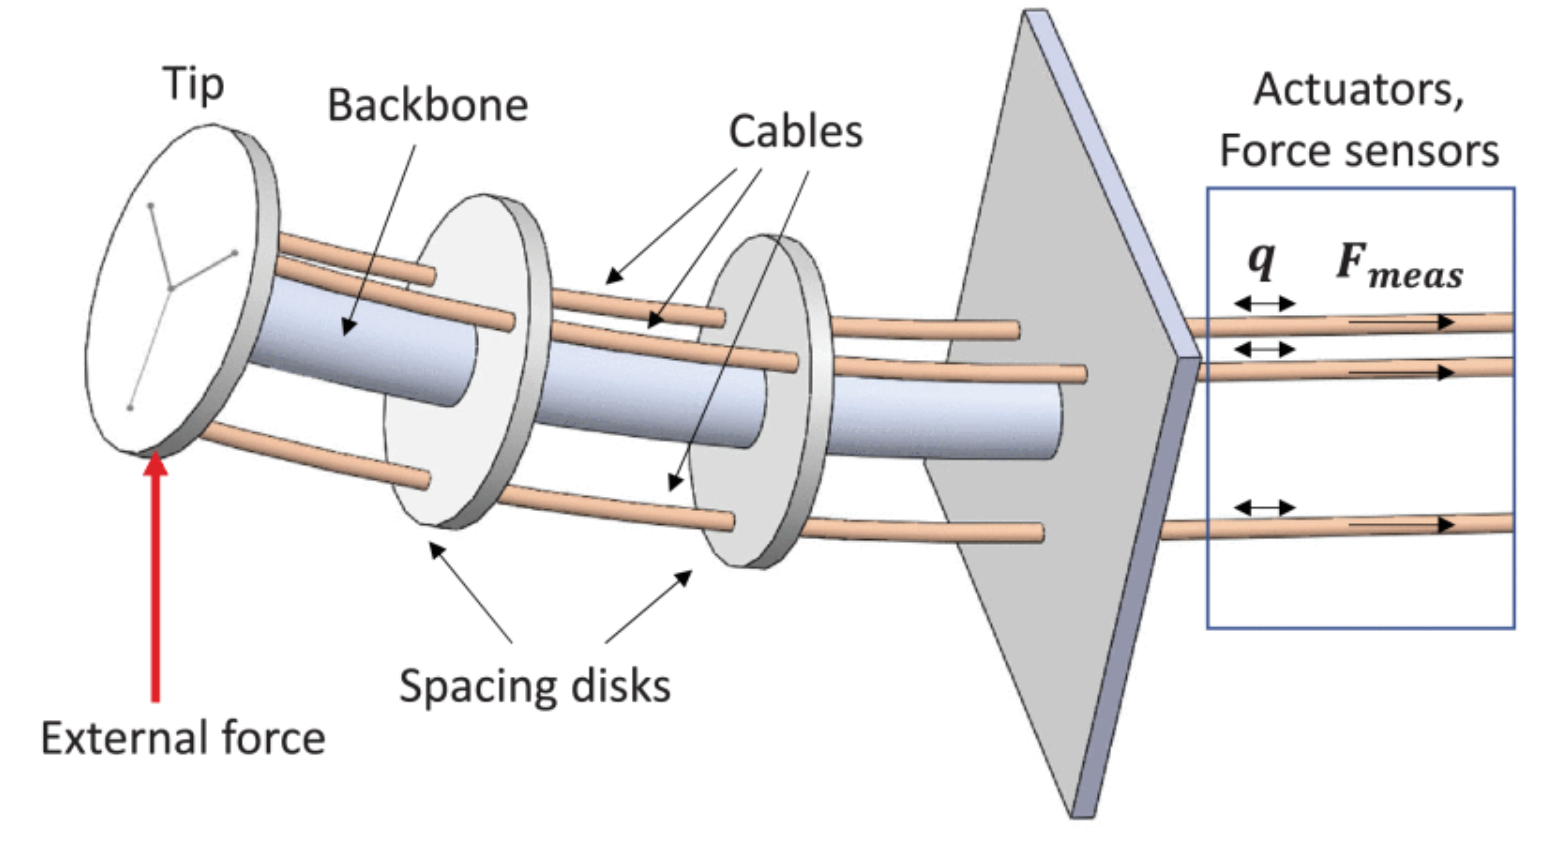
\includegraphics[width=.9\textwidth]{Image/LR/3tendon_1segment_CR.PNG} 
    \caption[The three tendons continuum robot with one segment]
    {\centering \textbf{The three tendons continuum robot with one segment} \cite{3tendon_1segment_CR}.}
    \label{fig:3tendon_1segment_CR}
\end{figure}
\noindent Figure \ref{fig:3tendon_1segment_CR} shows only the simplest tenon-driven robots. In practical applications, there 
may be more than one backbone, and the disks are not necessarily parallel. \\
Compared with other continuum robots, one of the most significant advantages of tendon-driven robots is their flexibility. 
This advantage makes it more effective in performing tasks in complex and restrictive Spaces. In addition, due to the simple 
components needed to construct the robot, it is easier to meet lightweight design specifications. Moreover, like the 
concentric-tube continuum robots, tendon-driven continuum robots can be built designed on a small scale with diameters of 
below 10mm \cite{amanov2021tendon}. \\
However, due to its simple actuating principle, more complex algorithms are needed to control it more accurately. Also, the 
tendon-driven robots actuate by pulling the tendon, which makes the friction between the tendon and other components inevitable, 
which will accelerate the wearing speed of the tendon-driven robots.
\subsubsection{Fishbone Robots}
Fishbone robots, as the name suggests, are inspired by fish bones. It is consists of several "fishbone moduless", which are 
composed of a number of rigid cross-shaped plates, and a flexible elastic plate backbone embedded in the middle, 
forming a rigid-soft coupling structure\cite{fishboneCR}. When the different modules are connected, the backbones of the bionic fishbone modules 
are perpendicular to each other, and finally form a complete main frame of the fishbone robot. Like the tendon-driven robot, 
the fishbone robot is also controlled by cable, but it is worth noting that each module is controlled by two separate 
cables. This means that for a fishbone robot composed of n fishbone modules, there are a total of 2n cables controlling the motion
of the whole robot. In addition, the planes formed by the two ropes that control each module are perpendicular to each other, so 
that each section rotates along a plane perpendicular to each other. 
\begin{figure}[H] %[H] "corresponds to start the figure Here" 
    \centering %alignment can be flushleft or flushright
    \captionsetup{labelsep=colon}
    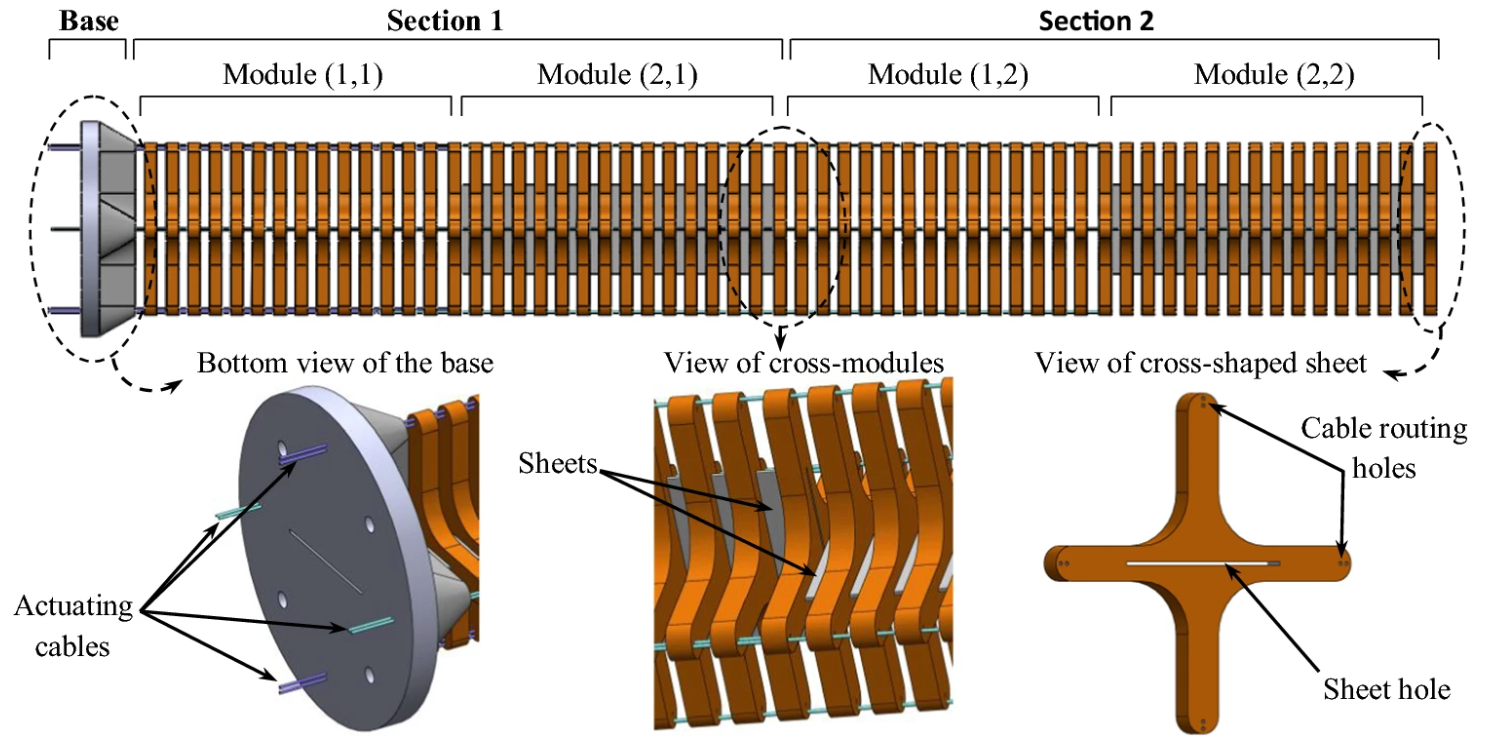
\includegraphics[width=.9\textwidth]{Image/LR/fishbone_CR_amouri2023bio.PNG} 
    \caption[The cable-driven fish bone continuum robot]
    {\centering \textbf{The cable-driven fish bone continuum robot with cable arrangement} \cite{amouri2023bio}.}
    \label{fig:fishboneCR_2023bio}
\end{figure}
\noindent From the graph above, it is shown that because of the numbers of rigid cross-shaped sheets formed a large diamater 
frame, the structural stability of this kind of robot is very strong. Also, each fishbone unit can provide one DoF, making it 
easy to reach a very high total DoF. However, due to the multiple-curves deformation trajectory, the fishbone robots are not 
suitable for situations where strict trajectory is required\cite{fishboneCR}.
\subsubsection{Concentric Tube Continuum Robots}
concentric tube robots, shaped like retractable walking sticks, consist of many tubes with decreasing diameters. Each tube is 
nested on top of the previous wider tube.  \\
The concentric robots are made of two parts: tubes and coaxial actuation units. The tubes are the main structural element of 
this robot and act as the backbone. The coaxial actuation unit consists of two motors which are responsible for rotation and 
translation movement respectively. Each tube is actuated by an independent coaxial actuation unit. 
\begin{figure}[H] %[H] "corresponds to start the figure Here" 
    \centering %alignment can be flushleft or flushright
    \captionsetup{labelsep=colon}
    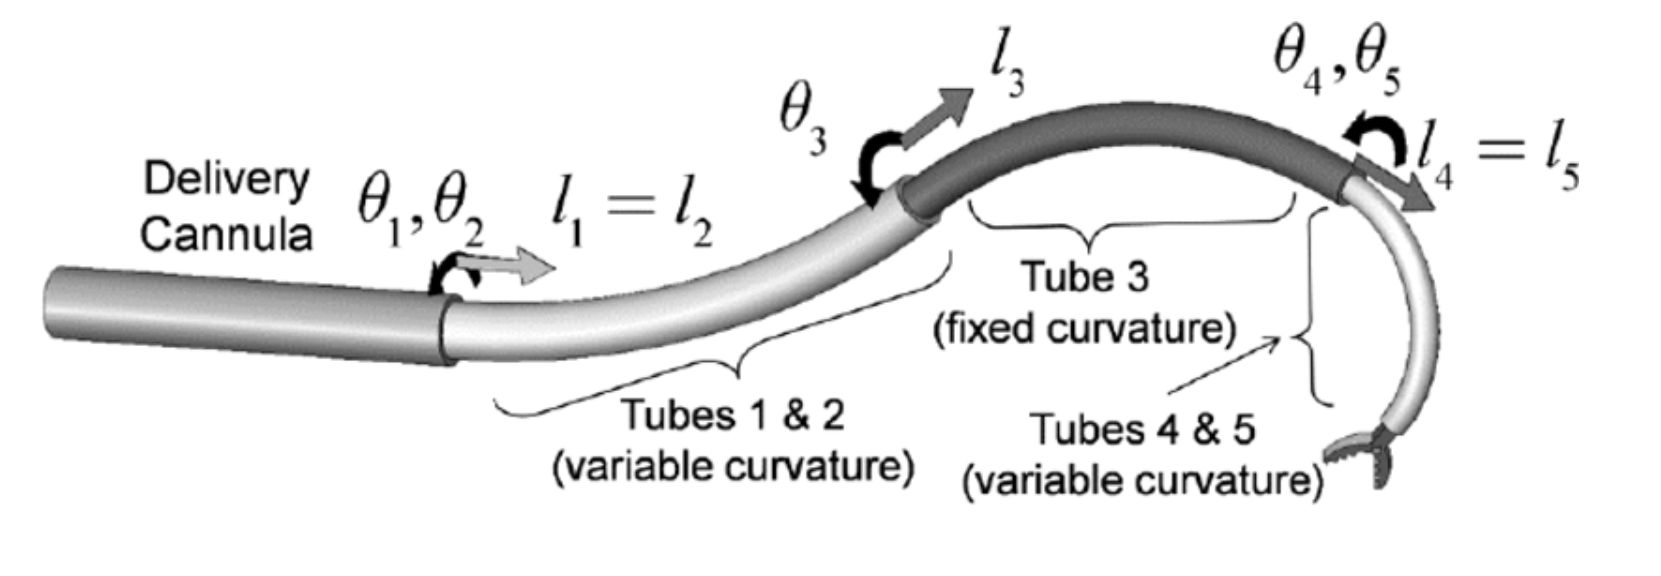
\includegraphics[width=.9\textwidth]{Image/LR/concentric_tube_CR.PNG} 
    \caption[An example concentric tube continuum robot]
    {\centering \textbf{An example concentric tube continuum robot} \cite{CTCR_example}.}
    \label{fig:CTCR_example}
\end{figure}
\noindent The most significant advantage of this kind of robots is that of all the continuum robots, concentric tube robots have the 
smallest possible outer diameter and are best suited to work in confined and narrow Spaces. Therefore, it is the ideal choice 
for surgical operations. \\
Their disadvantages, on the other hand, are also very evident. Since each tube requires an independent actuation unit, the 
overall length of the robot cannot be very long, because longer lengths will lead to more tubes, and will lead to more tip 
position errors.



% change to new page
\newpage % Literature Review
%%%%% Design %%%%%
\section{Design} 
This is the Design of the final report.
\subsection{part ??}
unknown
\subsection{part ??}
unknown
\subsection{part ??}
unknown

% change to new page
\newpage % Design
%%%%% Result and Discussion %%%%%
\section{Result and Discussion} 
%%%%% Strength Analysis %%%%%
\subsection{Strength Analysis}
\subsubsection{The Result of Strength Analysis}
The strength analysis conducted using ANSYS has yielded the following results.
\begin{itemize}
    \item Displacement \\
    The maximum displacement observed in the manipulator was 117.44 mm, located at the end-effector, which is shown 
    in Figure \ref{fig:displacement}.
    \begin{figure}[H] % figure
        \centering 
        \captionsetup{labelsep=colon}
        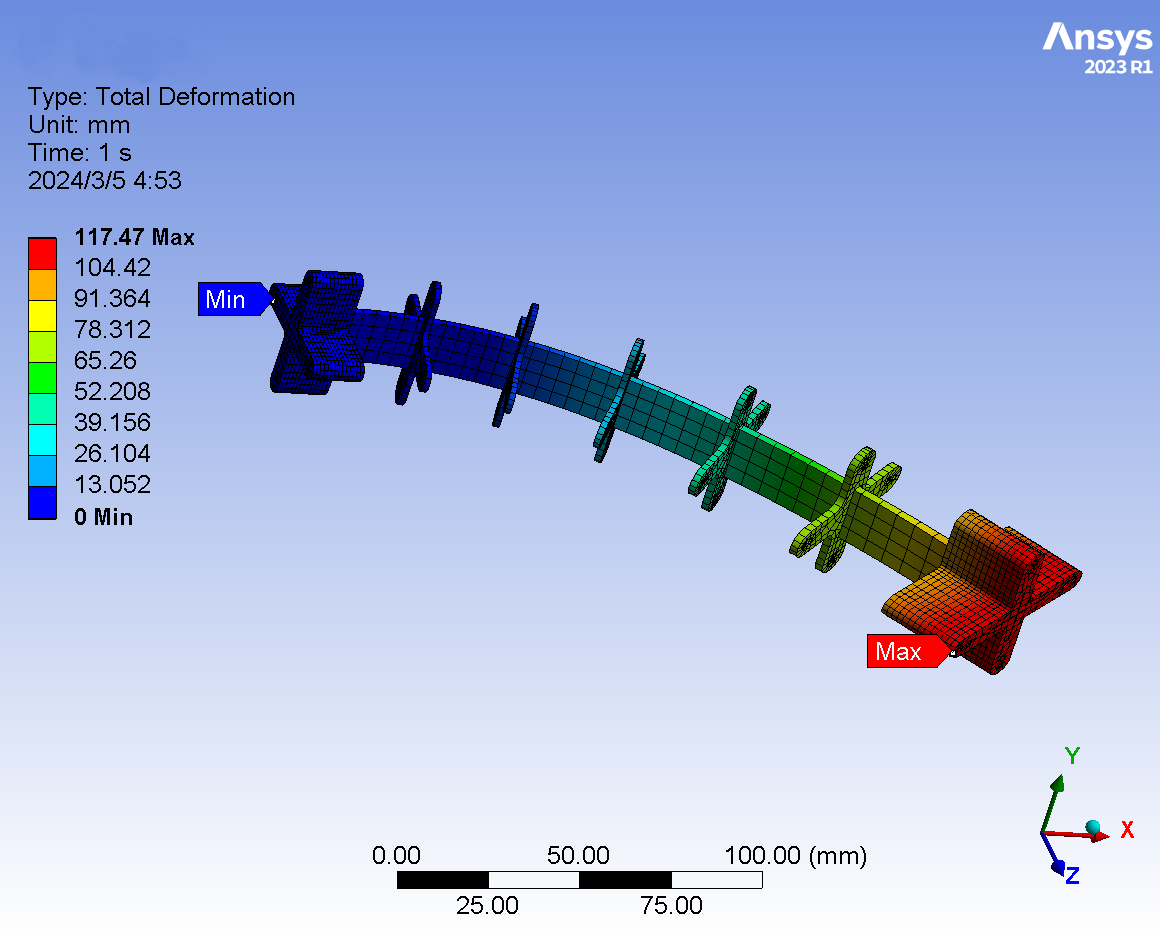
\includegraphics[width=0.75\textwidth]{Image/Result/displacement.png} 
        \caption[The displacement analysis of manipulator]
        {\centering \textbf{The displacement analysis of manipulator.}}
        \label{fig:displacement}
    \end{figure}
    \item Stress \\
    As shown in Figure \ref{fig:stress}, the maximum stress was found to be 476.63 MPa, occurring at the base of 
    elastic sheet where the manipulator experiences the most significant load. 
    \begin{figure}[H] % figure
        \centering 
        \captionsetup{labelsep=colon}
        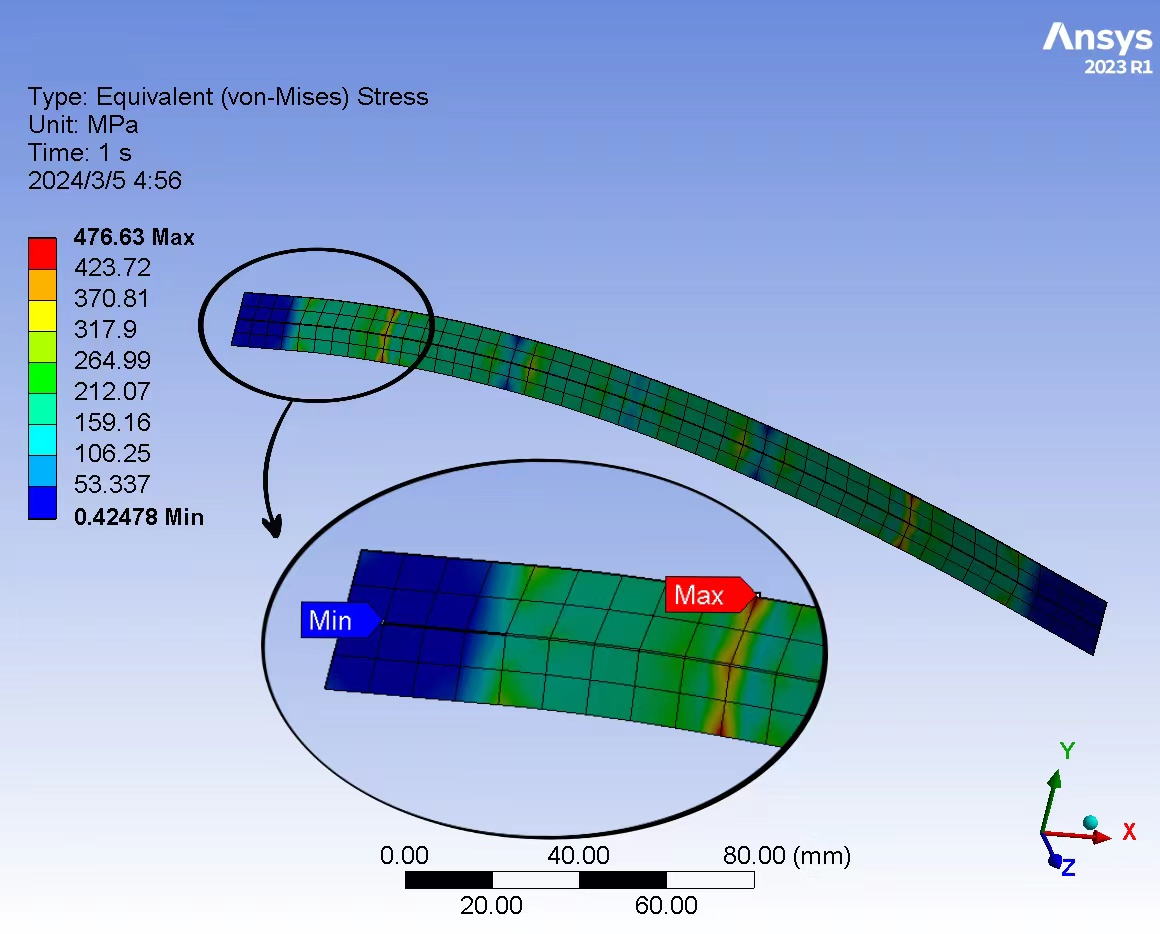
\includegraphics[width=0.75\textwidth]{Image/Result/stress.jpg} 
        \caption[The stress analysis of manipulator]
        {\centering \textbf{The stress analysis of manipulator.}}
        \label{fig:stress}
    \end{figure}
\end{itemize}
The results indicate that Maximum stress is concentrated on the elastic sheet of the manipulator near the 
connector, which suggests that this is the most likely location for failure under the current design and 
loading conditions. The maximum von Mises stress did not exceed the typical yield strength of 65Mn alloy 
teel, indicating that the arm would return to its original shape after the removal of the load and there is 
no potential risk of plastic deformation or failure. This enhances the arm's reliability and extends its 
operational lifespan. \\
Given that the material remains within its elastic limit, the design could potentially be optimized further 
to reduce weight or increase load capacity. Future work may explore these possibilities while maintaining 
the safety factors within the design criteria.
\subsubsection{Limitations and Solutions}
\begin{itemize}
    \item Simplification of the Model \\
    The initial analysis simplified the complex structure of the manipulator by focusing on a single module, 
    potentially overlooking critical interactions between various modules that contribute to the overall 
    strength and performance of the system. This simplification, while beneficial for computational efficiency, 
    may not accurately reflect the integrated behavior of the manipulator in real-world scenarios where interactions 
    between modules can significantly influence outcomes. 
    \textit{Solution}: Future analyses could incorporate the interactions between all modules to provide a more 
    comprehensive understanding of the manipulator's behavior under various conditions. Such an approach will 
    ensure a more accurate representation of the manipulator's behavior under various operational conditions, 
    leading to more reliable performance predictions and informed design decisions. 
    \item Failure Point Concentration \\
    Stress concentration at the base of the elastic sheet indicates a potential failure point but does not 
    account for fatigue or long-term wear. This oversight could underestimate the long-term durability of 
    the manipulator, potentially leading to unexpected maintenance issues or failure. \\
    \textit{Solution}: To address this gap, incorporating a detailed fatigue analysis into future work is 
    crucial. This analysis should evaluate the impact of repeated stress cycles on the manipulator's components 
    over extended periods. By understanding these effects, design modifications can be implemented to enhance 
    the durability and operational lifespan of the manipulator. The modifications could include optimizing 
    material selection, redesigning stress-prone areas to reduce concentration points, and introducing preventive 
    maintenance schedules based on predicted failure. 
    \item Impact of cables \\
    The analysis did not consider the impact of cable tension on the manipulator's strength. Cable tension 
    can significantly affect the manipulator's mechanical behavior. Neglecting this factor may lead to an 
    incomplete understanding of the manipulator's operational capabilities and potential failure modes. \\
    \textit{Solution}: Future analyses should integrate the effects of cable tension to achieve a more accurate 
    assessment of the manipulator's performance. This could involve modifying the existing model to include 
    boundary conditions that accurately represent the forces exerted by cables under various load scenarios. 
    Implementing dynamic simulations that account for variations in tension forces during different stages of 
    operation will further enhance the fidelity of the model. These improvements will enable a more nuanced 
    understanding of the manipulator's capabilities, assisting in the design of a more robust and reliable 
    system capable of withstanding the complexities of real-world applications. 
\end{itemize}
%%%%% Error Analysis %%%%%
\subsection{Error Analysis of Cross-Shaped Sheets}
At the early stage of the project, given that the number of cross-shape sheets in each module have an 
influence on the maximum bending angle $\boldsymbol{\alpha}_{max}$, which is an essential parameter of those which 
affect the workspace of the manipulator, hence the number of sheets should be determined by deriving 
the functions of both absolute error and relative error \cite{fishboneCR} against the number of sheets. The 
simulation results are shown in Figure \ref{fig:error_analysis}.
\begin{figure}[H] % figure
    \centering 
    \captionsetup{labelsep=colon}
    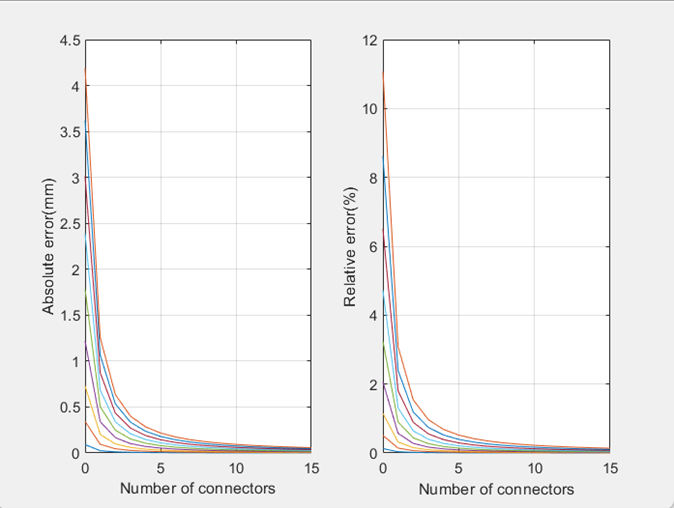
\includegraphics[width=0.8\textwidth]{Image/Result/error_analysis.png} 
    \caption[The simulation results of errors against the number of sheets]
    {\centering \textbf{The simulation results of errors against the number of sheets.}}
    \label{fig:error_analysis}
\end{figure}
\noindent As illustrated in Figure \ref{fig:error_analysis}, the changing trends of both absolute and 
relative errors are almost identical since 
the relative error is proportional to the absolute error, and the different lines with different colors represent 
the data with different bending angles whose range is from 10 degrees to 90 degrees in both directions (positive 
or negative). It is obvious that both errors decrease with the increase in the number of connecting sheets, hence 
theoretically, the number of sheets should be as large as possible to make both errors could be negligible. However, 
the number of sheets also has an influence on the size of simulation space, more the number of sheets less the size 
of simulation space given that if the length of manipulator is much longer, the space near to the basement of 
manipulator could not be reached due to the characteristics of the material. Hence, the number of sheets could be 
assumed to be 10 rather than 15, even though both the errors are smaller when the number of sheets is 15. 
%%%%% Workspace Analysis %%%%%
\subsection{Manipulator Workspace Analysis}
The workspace simulation of the manipulator has been illustrated since it is important to determine the 
variables of joints based on the required workspace. The segmented workspace is affected by several aspects, 
which include the simulation index and the range within the three-dimensional coordinates. The effective workspace 
of the manipulator is a cubic whose dimension is 300x300x300 (mm). The specific workspace has a fixed range on 
the x and y axes from -150 to 150 mm. Therefore, it is only necessary to determine the range of the workspace 
along the z-axis. The parameter H, representing the height of the basement of specific workspace, is 
utilized to determine the range of the workspace along the z-axis. The impacts of different indices and 
parameter H will be discussed separately, aiming to segment the appropriate cubic workspace of the manipulator.
\begin{figure}[H] % figure
    \centering 
    \captionsetup{labelsep=colon}
    \begin{subfigure}{0.45\textwidth} % subfigure 1
        \centering
        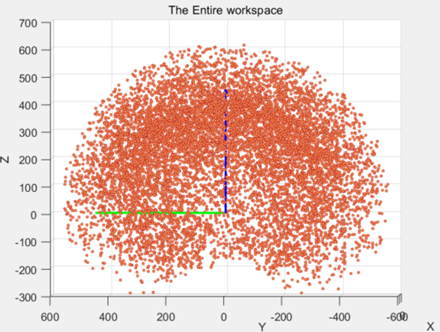
\includegraphics[width=\linewidth]{Image/Result/workspace_10000.png}
        \caption{\centering The entire workspace where simulation index=10000}
        \label{fig:ws_10000}
    \end{subfigure}
    \hfill
    \begin{subfigure}{0.45\textwidth} % subfigure 2
        \centering
        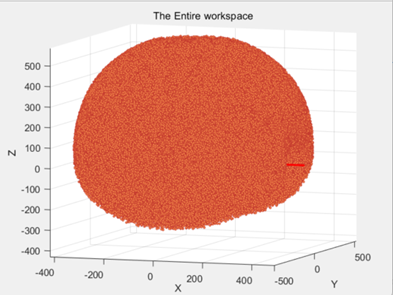
\includegraphics[width=\linewidth]{Image/Result/workspace_1000000.png}
        \caption{\centering The entire workspace where simulation index=1000000}
        \label{fig:ws_1000000}
    \end{subfigure}
    \caption[The entire workspace with different random indices]
    {\centering \textbf{The entire workspace with different simulation indices.}}
    \label{fig:ws_diff}
\end{figure}
\vspace{-5mm}
\noindent As shown in Figure \ref{fig:ws_10000}, the working space of manipulator forms a spherical shell-shaped 
point cloud consisting of 10000 floating points since the simulation index is 10000, which is insufficient to fully 
occupied the theoretical workspace. To further generalize the theoretical workspace, it is necessary to increase 
the simulation index. The appropriate workspace should be divided from the workspace whose index is 1000000. 
\begin{figure}[H] % figure
    \centering 
    \captionsetup{labelsep=colon}
    \begin{subfigure}{0.45\textwidth} % subfigure 2
        \centering
        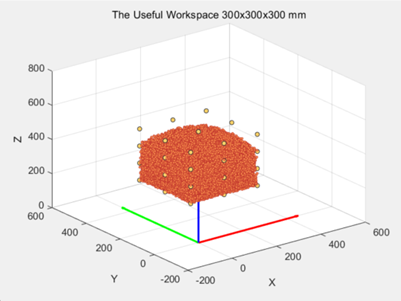
\includegraphics[width=\linewidth]{Image/Result/rect_workspace_1000000_350-650.png}
        \caption{\centering The cubic workspace of manipulator with index = 1000000 H=350-650 mm}
        \label{fig:ws_1000000_350}
    \end{subfigure}
    \hfill
    \begin{subfigure}{0.45\textwidth} % subfigure 1
        \centering
        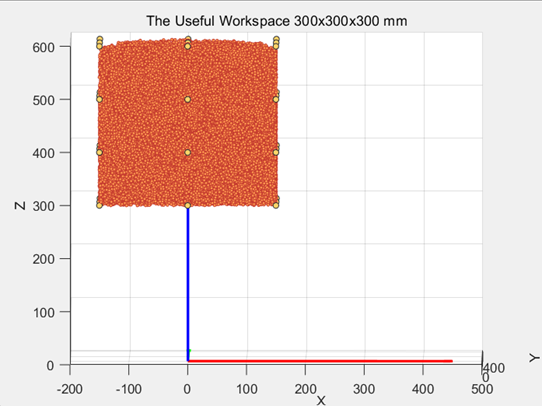
\includegraphics[width=\linewidth]{Image/Result/rect_workspace_1000000_300-600.png}
        \caption{\centering index = 1000000 H=300-600 mm}
        \label{fig:ws_10000_300}
    \end{subfigure}
    \caption[The cubic workspace with different segmentation]
    {\centering \textbf{The cubic workspace with different segmentation.}}
    \label{fig:ws_300_350}
\end{figure}
\vspace{-5mm}
\noindent Comparing the simulation results illustrated in Figure \ref{fig:ws_300_350}, it can be observed that the upper 
area of the segmented cubic workspace whose H=350mm failed to be occupied. However, the segmented cubic workspace 
whose H=300mm is almost fully occupied. To determine threshold of parameter H, a series of yellow detection points 
are utilized to test whether specific locations in the workspace can be reached. A programme is utilized to calculate 
the distance between the detection points and the simulated point cloud and identify the minimum distances. The  
simulation results whose index=1000000 and H=300mm are shown in Figure \ref{fig:matlab_300} in Appendix 
\ref{append:code_display}. The top view of the cubic workspace in Figure \ref{fig:top_view} associates labels with 
detection points, facilitating subsequent explanations. 
\begin{figure}[H] % figure
    \centering 
    \captionsetup{labelsep=colon}
    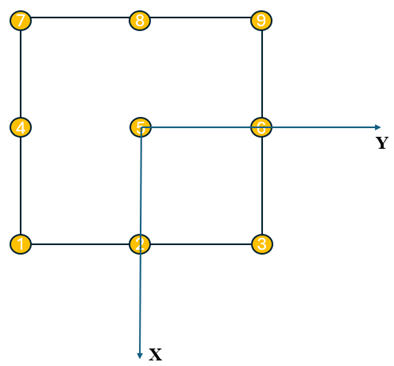
\includegraphics[width=0.5\textwidth]{Image/Result/top_view_rect_workspace.png} 
    \caption[The top view of the workspace and the labels of detection points]
    {\centering \textbf{The top view of the workspace and the labels of detection points.}}
    \label{fig:top_view}
\end{figure}
\vspace{-5mm}
\noindent While H=300 mm, The heights of the first, second, third, and fourth layers are 300 mm, 400 mm, 500 mm, and 600 mm, 
respectively. As the second and third layers are situated in the middle, theoretically all detection points on 
these two layers are reachable. Therefore, the mean and variance of distances to these points can be calculated. 
Combined with a normal distribution whose $\mu = 0$, a threshold is set to be 99.7\% of the data are within 3 
standard deviations of the mean can be derived to determine whether detection points on the first and fourth 
layers are reachable. The threshold $\tau$ can be calculated in Equation \ref{eq:threshold_reachable}. \\
\vspace{-5mm}
\begin{align}
    &\bar{d}_{2,3} = \sum_{i=2}^3 \sum_{j=1}^9 d_{ij,min} \nonumber \\
    &\sigma_{2,3}=\sqrt{\dfrac{1}{n}\times\sum_{i=1}^n(d_i-\bar{d})^2} \nonumber \\
    &\tau = \bar{d}_{2,3} + 3\times\sigma_{2,3}
    \label{eq:threshold_reachable}
\end{align}
The segmentation of the effective workspace for other values of H, specifically H=240, 260, and 280 mm, 
can also be performed using the same approach. The numerical values corresponding to different H parameters 
are illustrated in Figures \ref{fig:matlab_240}, \ref{fig:matlab_260}, \ref{fig:matlab_280} in Appendix 
\ref{append:code_display}. The results and reachability for different H are presented in Table 
\ref{tab:threshold_and_reachability}.
\begin{center}
    \small
    \begin{longtable}{l l l l l l }
    \caption{The Reachability of Detection Points with Different H.} \label{tab:threshold_and_reachability} \\
    \hline \multicolumn{1}{l}{\textbf{H (mm)}} & 
    \multicolumn{1}{l}{\textbf{Layer}} & 
    \multicolumn{1}{l}{\textbf{$\bar{d}_{2,3}$ (mm)}} & 
    \multicolumn{1}{l}{\textbf{$\sigma_{2,3}$ (mm)}} & 
    \multicolumn{1}{l}{\textbf{Threshold $\tau$ (mm)}} & 
    \multicolumn{1}{l}{\textbf{Reachability}} \\ \hline 
    \endfirsthead
    \multicolumn{6}{c}%
    {{\bfseries \tablename\ \thetable{} -- continued from previous page}} \\
    \hline \multicolumn{1}{l}{\textbf{H (mm)}} & 
    \multicolumn{1}{l}{\textbf{Layer}} & 
    \multicolumn{1}{l}{\textbf{$\bar{d}_{2,3}$}} & 
    \multicolumn{1}{l}{\textbf{$\sigma_{2,3}$}} & 
    \multicolumn{1}{l}{\textbf{Threshold $\tau$}} & 
    \multicolumn{1}{l}{\textbf{Reachability}} \\ \hline 
    \endhead
    \hline \multicolumn{6}{|r|}{{Continued on next page}} \\ \hline
    \endfoot
    \hline \hline
    \endlastfoot
    % table context
    300&1&5.79 & 2.50 & 13.29 &9 \\
       &4&5.79 & 2.50 & 13.29 &3 \\
    280&1&4.87 & 2.02 & 10.94 &9 \\
       &4&4.87 & 2.02 & 10.94 &4 \\
    260&1&5.37 & 2.01 & 11.41 &7 \\
       &4&5.37 & 2.01 & 11.41 &7 \\
    240&1&5.35 & 2.48 & 12.78 &8 \\
       &4&5.35 & 2.48 & 12.78 &9 \\
    \hline
    \end{longtable}
\end{center}
\vspace{-5mm}
As shown in Table \ref{tab:threshold_and_reachability}, setting H to 240 mm achieves better reachability, 
which is more reasonable compared to other scenarios. Additionally, to obtain a more accurate threshold, 
multiple tests or experimenting with a greater number of simulation indices can be undertaken to reduce random 
and systematic errors.
%%%%% INVERSE KINEMATICS %%%%%
\subsection{Inverse Kinematics}
This section will demonstrate the posture solution of single modules and trajectory replication results 
obtained through the IK algorithm. An in-depth analysis of accuracy and computational speed will be conducted, 
along with a discussion of its advantages and limitations. Using angles as input for the programme testing was 
preferred due to the complexity involved in specifying 12 indices of $\textbf{O}{target}$ and $\textbf{P}{target}$. 
%%%%% Singular Posture Solution %%%%%
\subsubsection{Posture Solution of Single Module Bending}
Firstly, the bending of individual modules was tested as the target for the IK solution. The 
IK algorithm was tested for different angles of bending for Modules 1, 2, 3, and 4, and the 
specific results are presented in Table \ref{tab:single_posture_IK} in Appendix \ref{append:table}. The 
solutions of the Modules 3 and 4 were highly satisfactory, with Module 3 even converging to an error of 0.02 mm 
in 6 epochs. However, the results of the Modules 1 and 2 were unsatisfactory, which were caused by inappropriate 
initialization. According to the flowchart in Figure \ref{fig:flowchart}, the IK algorithm requires an 
initialization to start iterations. Take the example of the target with 
$\boldsymbol{\alpha} = [0,\ 90,\ 0,\ 0]\degree$, after initializing with the initial posture in Figure 
\ref{fig:kinematics model 0_0_0_0} and applying the IK algorithm for iterations, the first iteration yielded 
a posture with 
$\boldsymbol{\theta} = [-0.0,\ 104.04,\ -0.0,\ -22.0]\degree$. Moreover, since each iteration starts from Module 4, 
the error in Module 4 cannot be eliminated. To mitigate this effect, selecting a more suitable posture for 
initialization is crucial. If the posture used for initialization with 
$\boldsymbol{\alpha} = [0,\ 100,\ 0,\ 0]\degree$, the solution of the IK algorithm would change to 
$\boldsymbol{\theta} = [-0.0,\ 81.77,\ -0.0,\ 9.3]\degree$. Nevertheless, due to errors generated by the 
iteration sequence, complete elimination remains challenging, and efforts were make to minimize the error to the 
greatest extent possible.  \\
Afterwards, the complex bending angles of modules was utilized as the target to investigate the influences of initialization. 
The target with angles $\boldsymbol{\alpha} = [80,\ 120,\ -120,\ 90]\degree$ was selected because its solution is complex, 
and it lies within the workspace of manipulator. The posture of the manipulator is shown in Figure 
\ref{fig:complex_target}. This scenario is likely to occur in practical applications and necessitates resolution 
through relevant methods. \\
With the initialization using the initial posture, the solution was 
$\boldsymbol{\theta} = [-8.88, -89.99, -126.81, -169.73]\degree$, which is shown in Figure \ref{fig:complex_init_0_0_0_0}. 
However, the solution of IK algorithm was $\boldsymbol{\theta} = [84.98,\ 122.93,\ -114.9,\ 63.01]\degree$, 
which is significantly close to the target while the angles for initialization were $[85,\ 125,\ -115,\ 55]\degree$. 
The solution of the IK algorithm with more appropriate initialization is shown in Figure 
\ref{fig:complex_init_85_125_-115_55}. This signifies that if the manipulator is presently in a posture similar 
to the target configuration, it can accurately determine the corresponding bending angles $\boldsymbol{\theta}$ through the 
IK algorithm. This proved to be highly beneficial for trajectory replication. 
\begin{figure}[H] % figure
    \centering 
    \captionsetup{labelsep=colon}
    \begin{subfigure}{0.9\textwidth} % subfigure 1
        \centering
        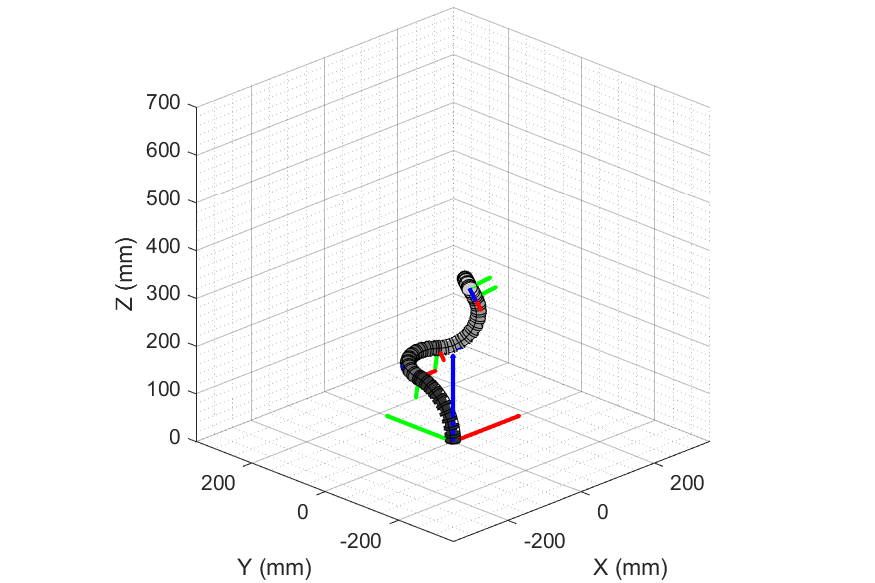
\includegraphics[width=\linewidth]{Image/MATLAB/manipulator_80_120_-120_90.png}
        \caption{\centering target: $\boldsymbol{\alpha} = [80,\ 120,\ -120,\ 90] \degree$ \\ \qquad}
        \label{fig:complex_target}
    \end{subfigure}
    \begin{subfigure}{0.49\textwidth} % subfigure 2
        \centering
        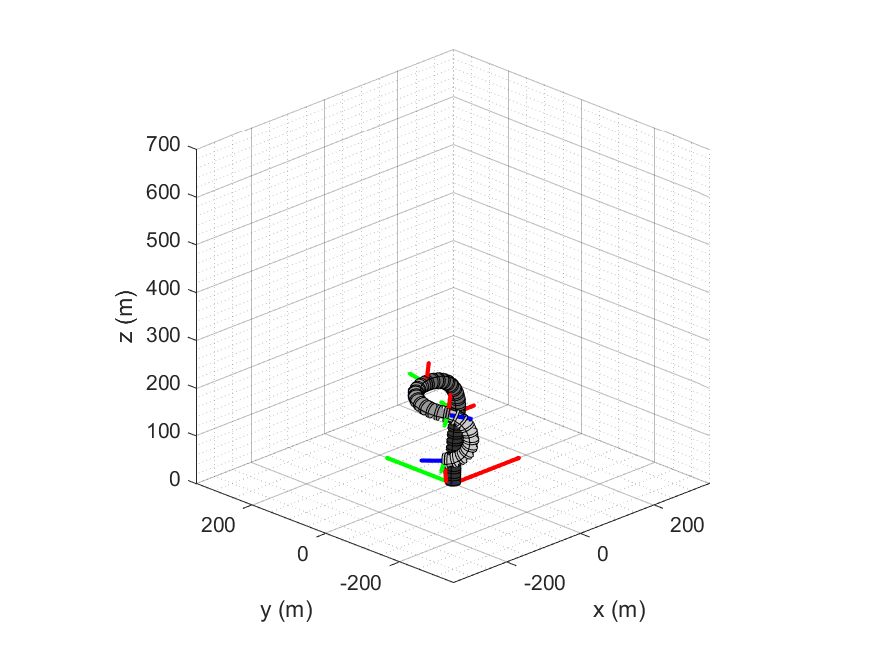
\includegraphics[width=\linewidth]{Image/MATLAB/manipulator_-8.88_-89.99_-126.81_-169.73.png}
        \caption{\centering initialization: $\boldsymbol{\alpha} = [0, 0, 0, 0]\degree$; \\
        $\boldsymbol{\theta} = [-8.88,\ -89.99,\ -126.81,\ -169.73]\degree$ }
        \label{fig:complex_init_0_0_0_0}
    \end{subfigure}
    \begin{subfigure}{0.49\textwidth} % subfigure 3
        \centering
        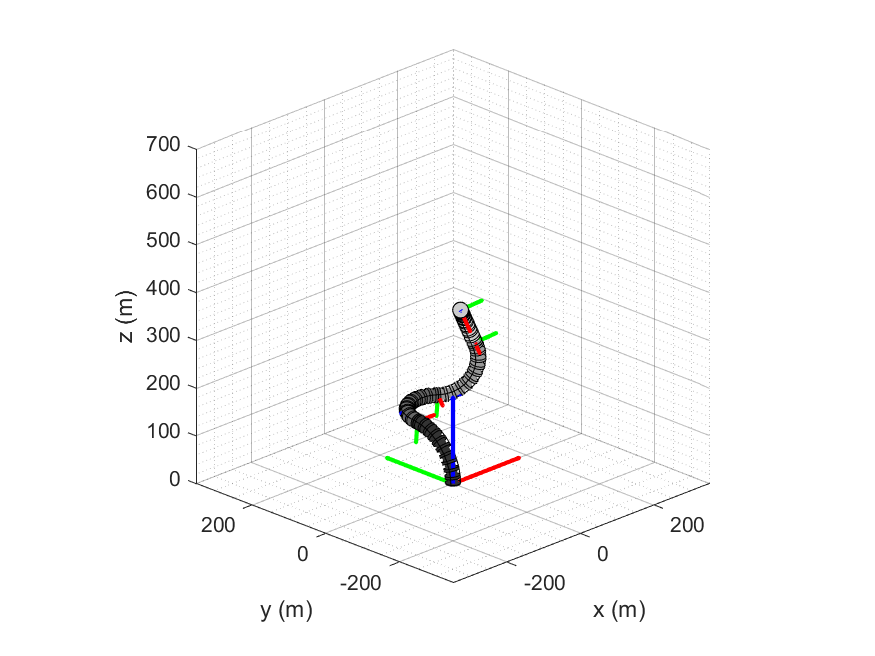
\includegraphics[width=\linewidth]{Image/MATLAB/manipulator_84.98_122.93_-114.9_63.01.png}
        \caption{\centering initialization: $\boldsymbol{\alpha} = [85, 125, -115, 55]\degree$; \\
        $\boldsymbol{\theta} = [84.98,\ 122.93,\ -114.9,\ 63.01]\degree$ }
        \label{fig:complex_init_85_125_-115_55}
    \end{subfigure}
    \caption[The kinematics model of manipulator with respective bending modules]
    {\centering \textbf{The inverse kinematics algorithm with different initialization.}}
    \label{fig:80_120_-120_90_diff_initial}
\end{figure}
\vspace{-5mm}
\noindent With the initialization using the initial posture, the solution was $\boldsymbol{\theta}$ = 
[-8.88, -89.99, -126.81, -169.73]$\degree$, which is shown in Figure \ref{fig:complex_init_0_0_0_0}. 
However, the solution of IK algorithm was $\boldsymbol{\theta} = [84.98,\ 122.93,\ -114.9,\ 63.01]\degree$, 
which is significantly close to the target while the angles for initialization were $[85,\ 125,\ -115,\ 55]\degree$. 
The solution of the IK algorithm with more appropriate initialization is shown in Figure 
\ref{fig:complex_init_85_125_-115_55}. This signifies that if the manipulator is presently in a posture similar 
to the target configuration, it can accurately determine the corresponding bending angles $\boldsymbol{\theta}$ through the 
IK algorithm. This proved to be highly beneficial for trajectory replication. \\
Ultimately, The efficient computational capability of algorithm is one of its strengths. The algorithm only 
took 1.905 seconds to complete 10,000 epochs updating. In practical applications, it requires only 200 epochs 
to determine convergence. In comparison to traditional methods like inverse Jacobian \cite{inverse_jacobian}, 
which involve matrix transformations and derivatives, this approach provides potential solutions in a short 
time, addressing the issue of singular points. However, this method has its limitations. In scenarios with 
multiple segments, the algorithm may introduce significant errors due to the iteration order, and these errors 
were difficult to be eliminated. The only viable solution is to enhance the algorithm's performance through 
suitable initialization methods.
%%%%% Trajectory Replication %%%%%
\subsubsection{Trajectory Replication}
The preceding discussion has highlighted genetic method, which is utilizing the current posture for 
initialization in trajectory replication. In this phase, a comparison of different initializations aimed to 
highlight the benefits of incorporating genetic method in trajectory replication and planning for the IK 
algorithm. Subsequently, the genetic method and IK algorithm are employed to 
replicate two types of trajectories: arc segments and closed paths. This section will analyze the genetic 
method and these two trajectories, elucidating the strengths and weaknesses of inverse kinematics algorithm. \\
The blue trajectory in Figure \ref{fig:genetic_approach} is the target trajectory, which bending from 
$\boldsymbol{\alpha} = [0,\ 0,\ 0,\ 0]$ to $\boldsymbol{\alpha} = [20,\ 20,\ 20,\ 20]$ equally in 20 steps. 
The red and purple trajectories are the replications using consistent initialization method and the genetic 
initialization method, respectively. The trajectory replication using the genetic method was comparatively better 
aligned with the target. The corrective effectiveness of the genetic algorithm was validated for 
other targets. The data of trajectories in Figure \ref{fig:genetic_approach} is listed in Table 
\ref{tab:trajectory_with_without_genetic}.
\begin{figure}[H] % figure
    \centering 
    \captionsetup{labelsep=colon}
    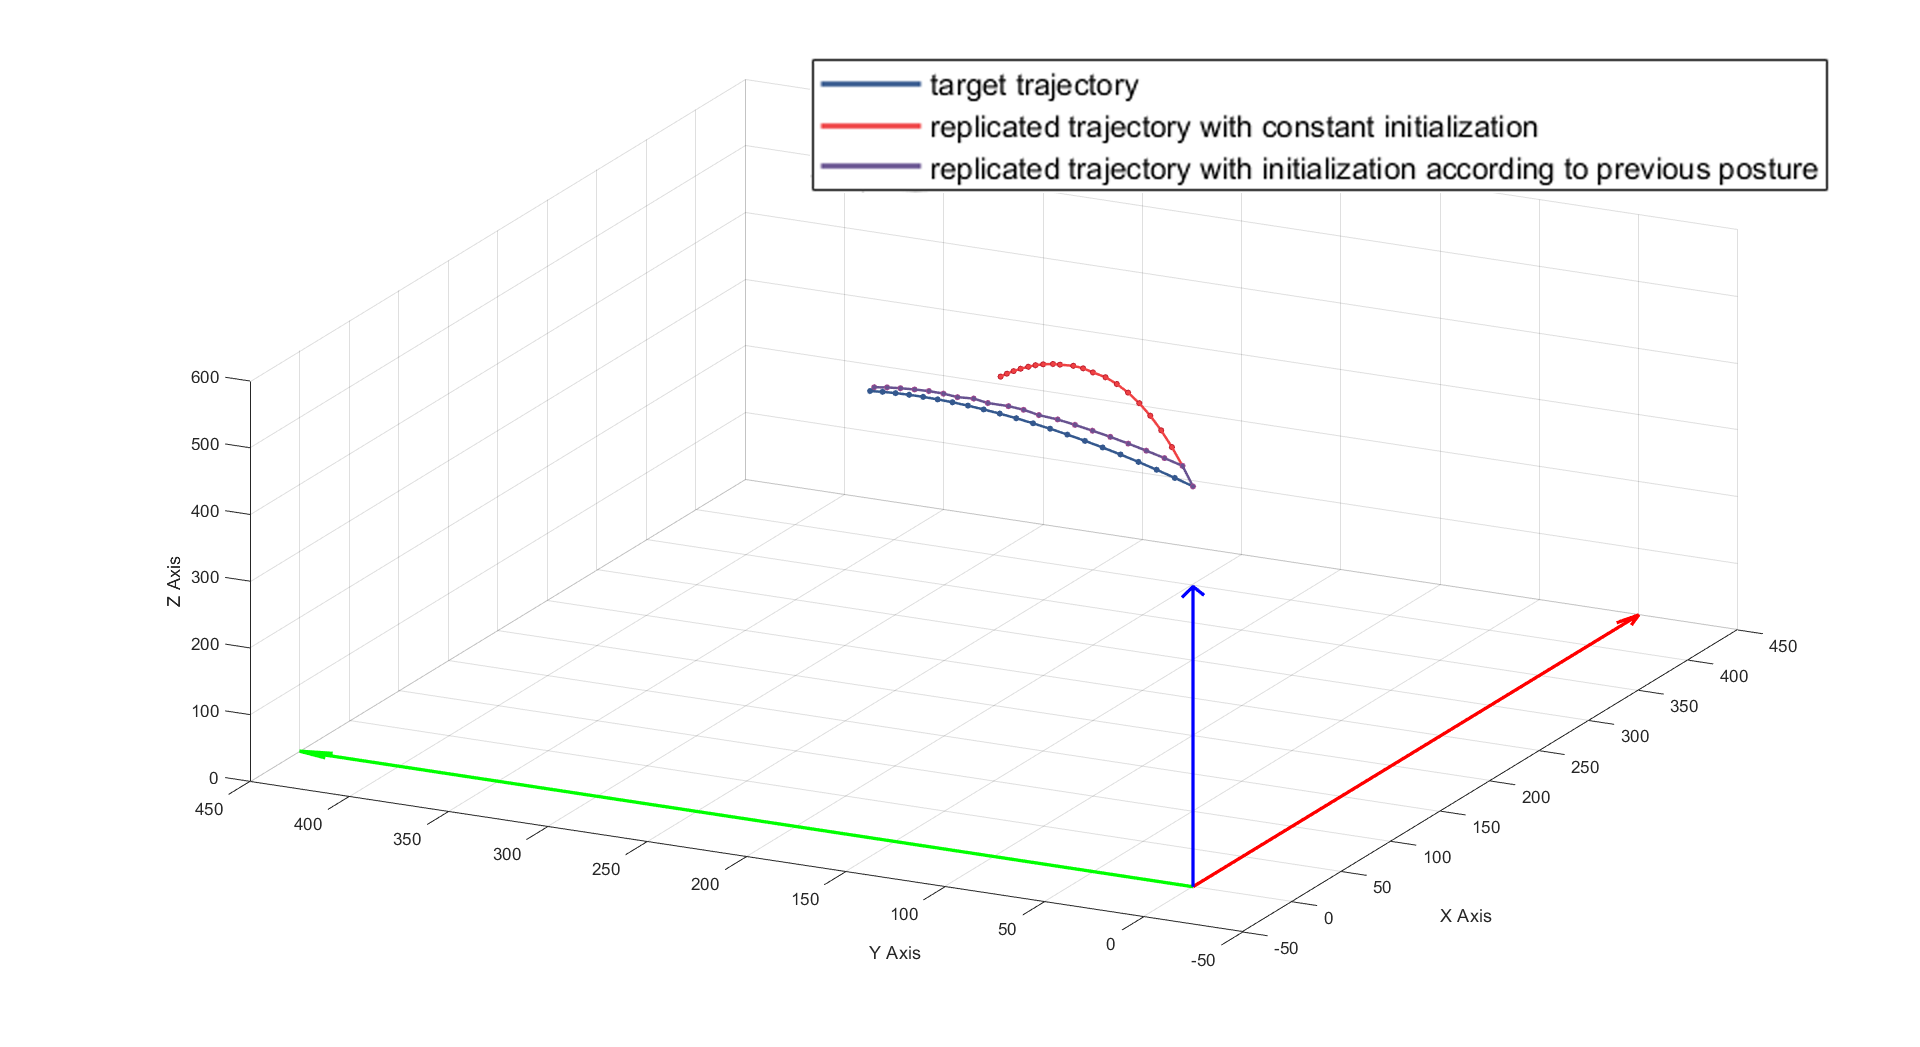
\includegraphics[width=1.0\textwidth]{Image/Result/trajectory_replication_diff_initialization.png} 
    \caption[The trajectory replications with and without genetic method]
    {\centering \textbf{The trajectory replications with and without genetic method.}}
    \label{fig:genetic_approach}
\end{figure}
\vspace{-5mm}
\noindent The replicated trajectories of both target trajectories closely align, but there exists a certain degree of error. 
This discrepancy was attributed to the inclusion of the error threshold $\boldsymbol{\epsilon}$ set at 0.02 in the 
programme, allowing for computational efficiency while maintaining accuracy. However, when dealing with significantly 
larger angular deviations, instances may arise where the replicated trajectories failed to precisely match the 
target trajectories. This situation was overlooked as it fell beyond the defined workspace. The average errors
about the trajectory replication were calculated in Table \ref{tab:traj_average_errors}.
\vspace{-5mm}
\begin{center}
    \small
    \begin{longtable}{l l l}
    \caption{The Average Errors of the replicated trajectories.} \label{tab:traj_average_errors} \\
    \hline \multicolumn{1}{l}{\textbf{Replicated Trajectory}} & 
    \multicolumn{1}{l}{\textbf{$e_{average}$ (mm)}} & 
    \multicolumn{1}{l}{\textbf{$e_{average}$ (mm)}} \\ \hline 
    \endfirsthead
    \multicolumn{3}{c}%
    {{\bfseries \tablename\ \thetable{} -- continued from previous page}} \\
    \hline \multicolumn{1}{l}{\textbf{Replicated Trajectory}} & 
    \multicolumn{1}{l}{\textbf{$e_{average}$ (mm) of Figure \ref{fig:tr_cross}}} & 
    \multicolumn{1}{l}{\textbf{$e_{average}$ (mm) of Figure \ref{fig:tr_cross}}} \\ \hline 
    \endhead
    \hline \multicolumn{3}{|r|}{{Continued on next page}} \\ \hline
    \endfoot
    \hline \hline
    \endlastfoot
    % table context
    \textbf{total}	& 3.576157 & 6.415941 \\
    \textbf{in workspace}	& 1.032255 & 2.642474 \\
    \hline
    \end{longtable}
\end{center}
\begin{figure}[H] % figure
    \centering 
    \captionsetup{labelsep=colon}
    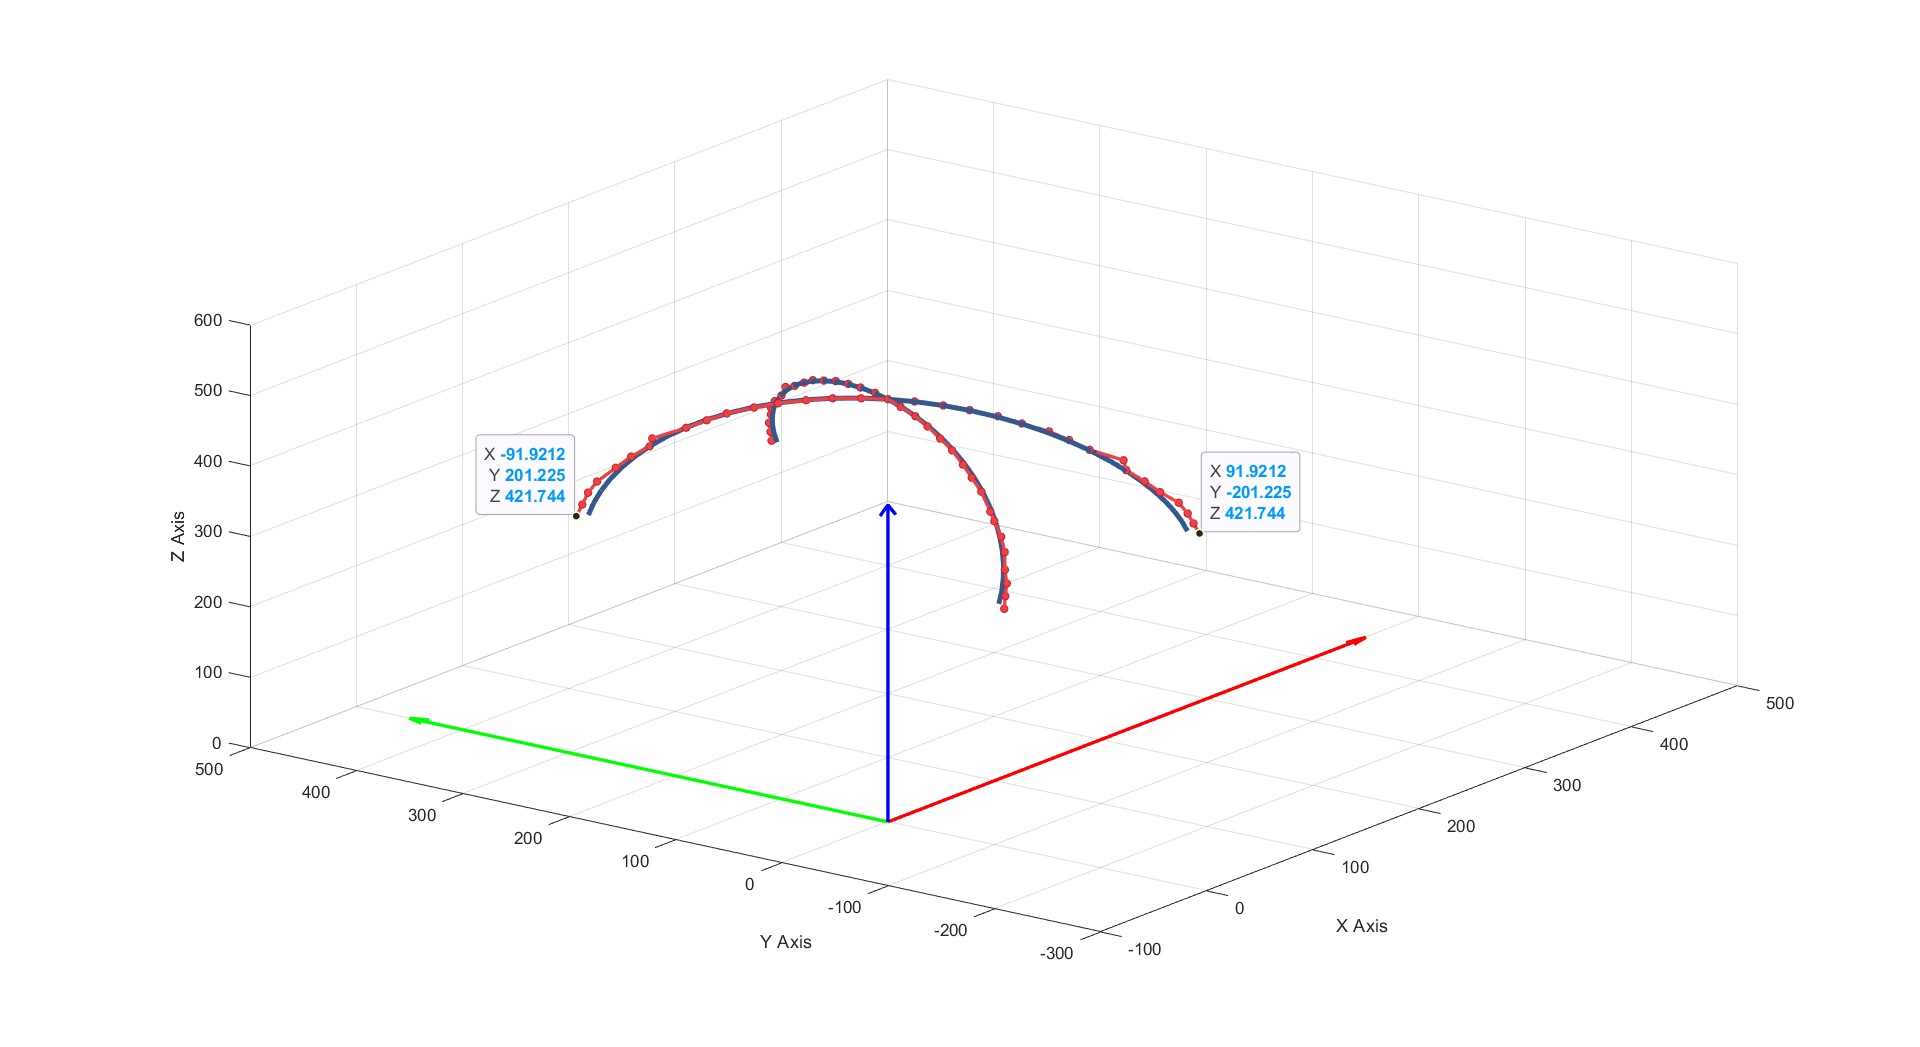
\includegraphics[width=1.0\textwidth]{Image/Result/cross_trajectory_replication_with_label.png} 
    \caption[The cross-shaped trajectory and its replication by IK algorithm]
    {\centering \textbf{The cross-shaped trajectory and its replication.}}
    \label{fig:tr_cross}
\end{figure}
\begin{figure}[H] % figure
    \centering 
    \captionsetup{labelsep=colon}
    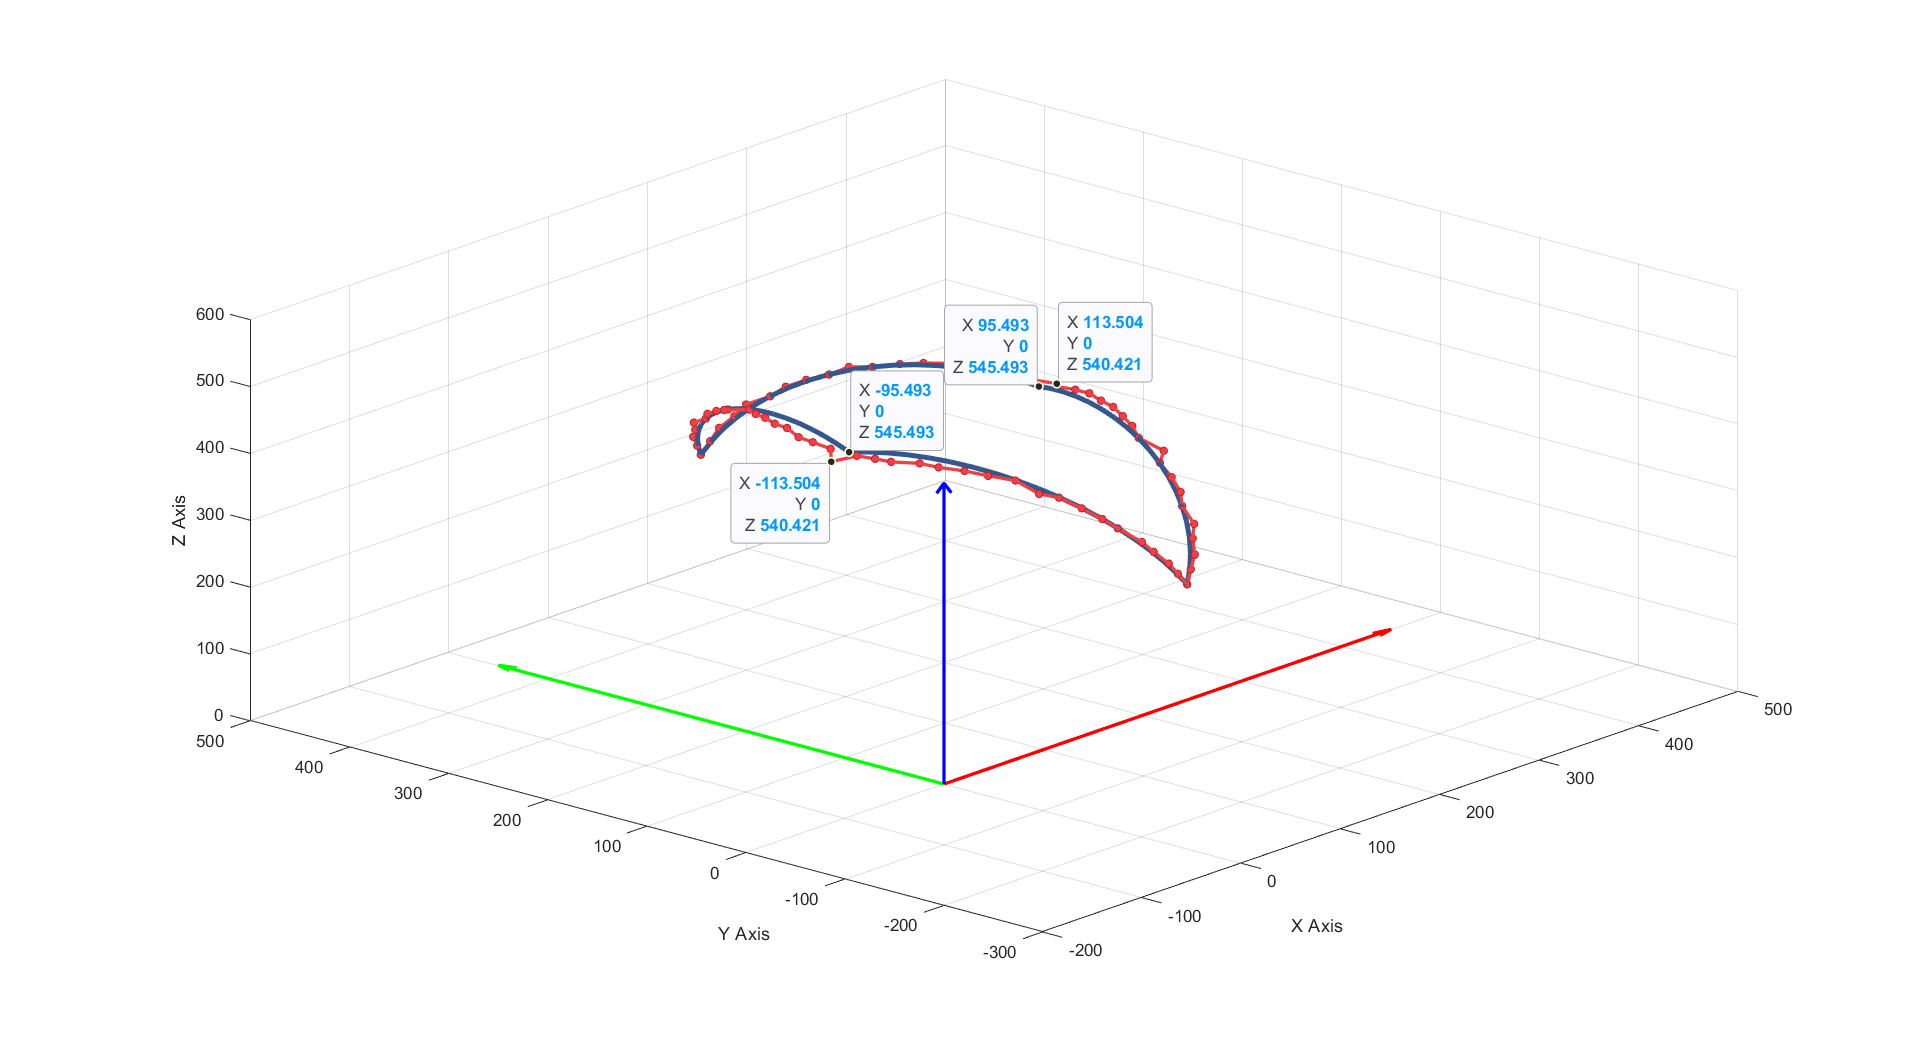
\includegraphics[width=1.0\textwidth]{Image/Result/circle_trajectory_replication_with_label.png} 
    \caption[The closed trajectory and its replication by IK algorithm]
    {\centering \textbf{The closed trajectory and its replication.}}
    \label{fig:clc_cross}
\end{figure}
%%%%% Limitation and Improvement %%%%%
\subsubsection{Limitation and Improvement}
However, it is challenging to calculate certain postures with IK algorithm. A method has 
been proposed involving continuous posture updating through a factor $f_u$. Nevertheless, this approach 
lacks systematic validation and is currently feasible only in specific circumstances. Therefore, it is 
mentioned here solely as a potential solution. \\
In practical applications, the initialization can be started with a relatively similar posture. 
In this context, the target where $\boldsymbol{\theta_{target}}$ = 
[45, 45, -45, -45] $\degree$ and the initialization with $\boldsymbol{\alpha_0}$ = [20, 20, -20, -20] $\degree$ 
were utilized to exemplify the corresponding calculations. The $\boldsymbol{target}$ is the position and 
orientation of the manipulator end effector. \\
The current posture with $\boldsymbol{\alpha_0}$  = [20, 20, -20, -20] $\degree$ was used as an initialization 
for calculations through inverse kinematics algorithm, resulting in the solution $\boldsymbol{\theta_1}$. 
The difference between $\boldsymbol{\alpha_0}$ and $\boldsymbol{\theta_1}$ was calculated by $f_u = 0.5$ to acquire 
$\boldsymbol{\alpha_1}$, which is shown in Equation \ref{eq:alpha_0_to_1}.
\begin{align}
    &\boldsymbol{\theta_1} = \textbf{FABRIKc}(\boldsymbol{target}, \boldsymbol{\alpha_0}) 
    = [42.38, 73.25, -69.59, -62.85]\degree \nonumber \\
    &\boldsymbol{\alpha_1} = \boldsymbol{\alpha_0} + f_u \cdot (\boldsymbol{\theta_1} - \boldsymbol{\alpha_0}) 
    = [31.19, 46.63, -34.80, -41.43]\degree
    \label{eq:alpha_0_to_1}
\end{align}
The $\boldsymbol{\alpha_i}$ can be continuously updated according to the method, which the results yield in Equations 
\ref{eq:alpha_1_to_2},\ref{eq:alpha_2_to_3}, \ref{eq:alpha_3_to_4}, \ref{eq:alpha_4_to_5}, and \ref{eq:alpha_5_to_6}.
\begin{align}
    &\boldsymbol{\theta_2} = \textbf{FABRIKc}(\boldsymbol{target}, \boldsymbol{\alpha_1}) 
    = [56.95, 34.48, -56.40, -38.96]\degree \nonumber \\
    &\boldsymbol{\alpha_2} = \boldsymbol{\alpha_1} + f_u \cdot (\boldsymbol{\theta_2} - \boldsymbol{\alpha_1}) 
    = [44.07, 40.56, -45.60, -40.20]\degree
    \label{eq:alpha_1_to_2}
\end{align}
\vspace{-18mm}
\begin{align}
    &\boldsymbol{\theta_3} = \textbf{FABRIKc}(\boldsymbol{target}, \boldsymbol{\alpha_2}) 
    = [43.64, 51.49, -45.97, -48.84]\degree \nonumber \\
    &\boldsymbol{\alpha_3} = \boldsymbol{\alpha_2} + f_u \cdot (\boldsymbol{\theta_3} - \boldsymbol{\alpha_2}) 
    = [43.56, 46.03, -45.79, -44.52]\degree
    \label{eq:alpha_2_to_3}
\end{align}
\vspace{-18mm}
\begin{align}
    &\boldsymbol{\theta_4} = \textbf{FABRIKc}(\boldsymbol{target}, \boldsymbol{\alpha_3}) 
    = [46.22, 42.71, -45.9, -43.88]\degree \nonumber \\
    &\boldsymbol{\alpha_4} = \boldsymbol{\alpha_3} + f_u \cdot (\boldsymbol{\theta_4} - \boldsymbol{\alpha_3}) 
    = [44.89, 44.37, -45.85, -44.20]\degree
    \label{eq:alpha_3_to_4}
\end{align}
\vspace{-18mm}
\begin{align}
    &\boldsymbol{\theta_5} = \textbf{FABRIKc}(\boldsymbol{target}, \boldsymbol{\alpha_4}) 
    = [44.87, 45.23, -45.03, -45.30]\degree \nonumber \\
    &\boldsymbol{\alpha_5} = \boldsymbol{\alpha_4} + f_u \cdot (\boldsymbol{\theta_5} - \boldsymbol{\alpha_4}) 
    = [44.88, 44.80, -45.85, -44.20]\degree
    \label{eq:alpha_4_to_5}
\end{align}
\vspace{-18mm}
\begin{align}
    &\boldsymbol{\theta_6} = \textbf{FABRIKc}(\boldsymbol{target}, \boldsymbol{\alpha_5}) 
    = [45.08, 44.91, -45.09, -44.96]\degree \nonumber \\
    &\boldsymbol{\alpha_6} = \boldsymbol{\alpha_5} + f_u \cdot (\boldsymbol{\theta_6} - \boldsymbol{\alpha_5}) 
    = [44.94, 44.86, -45.47, -44.58]\degree
    \label{eq:alpha_5_to_6}
\end{align}
\noindent In addition, another approach involves manually adjusting the manipulator's posture through observation, 
which is relatively straightforward but lacks precision. It is important to note that due to orientation constraints, 
the sum of angles for modules 1 and 3 and modules 2 and 4 should remain constant during the adjustment process.
%%%%% ELECTRONIC CONTROL %%%%%
\subsection{Electronic Control}
%%%%% Actuation Control %%%%%
\subsubsection{Actuation Control}
Initially, the testing of the results was supposed to be carried out through Proteus simulation. However, 
it was discovered that during the simulation process in Proteus, the motor components did not function normally, 
with frequent occurrences of stepping errors. Meanwhile, the simulation could not be completed in real-time 
due to the heavy load on the computer CPU. After consideration, the team members purchased a complete set of real 
components for testing. In the real circuit, the pin that each motor occupies are listed in Table \ref{tab:stepmotor_pin} 
to reduce the complexity of wiring. 
\vspace{-5mm}
\begin{center}
    \small
    \begin{longtable}{c c c c c c c c c}
    \caption{The Pin Assignment of Stepper Motors.} \label{tab:stepmotor_pin} \\
    \hline \multicolumn{1}{l}{\textbf{Stepper Motor}} & 
    \multicolumn{1}{l}{\textbf{1}} & 
    \multicolumn{1}{l}{\textbf{2}} & 
    \multicolumn{1}{l}{\textbf{3}} & 
    \multicolumn{1}{l}{\textbf{4}} & 
    \multicolumn{1}{l}{\textbf{5}} & 
    \multicolumn{1}{l}{\textbf{6}} & 
    \multicolumn{1}{l}{\textbf{7}} & 
    \multicolumn{1}{l}{\textbf{8}} \\ \hline 
    \endfirsthead
    \multicolumn{9}{c}%
    {{\bfseries \tablename\ \thetable{} -- continued from previous page}} \\
    \hline \multicolumn{1}{l}{\textbf{Stepper Motor}} & 
    \multicolumn{1}{l}{\textbf{1}} & 
    \multicolumn{1}{l}{\textbf{2}} & 
    \multicolumn{1}{l}{\textbf{3}} & 
    \multicolumn{1}{l}{\textbf{4}} & 
    \multicolumn{1}{l}{\textbf{5}} & 
    \multicolumn{1}{l}{\textbf{6}} & 
    \multicolumn{1}{l}{\textbf{7}} & 
    \multicolumn{1}{l}{\textbf{8}} \\ \hline 
    \endhead
    \hline \multicolumn{9}{|r|}{{Continued on next page}} \\ \hline
    \endfoot
    \hline \hline
    \endlastfoot
    % table context
    \textbf{Pin} &22&30&38&46&23&31&39&47 \\
    \textbf{Pin} &24&32&40&48&25&33&41&49 \\
    \textbf{Pin} &26&34&42&50&27&35&43&51 \\
    \textbf{Pin} &28&36&44&52&29&37&45&53 \\
    \hline
    \end{longtable}
\end{center}
\vspace{-15mm}
After connecting the Arduino to the stepper motors as depicted in Figure \ref{fig:circuit_connection}, 
the programme is ready for execution.
\begin{figure}[H] % figure
    \centering 
    \captionsetup{labelsep=colon}
    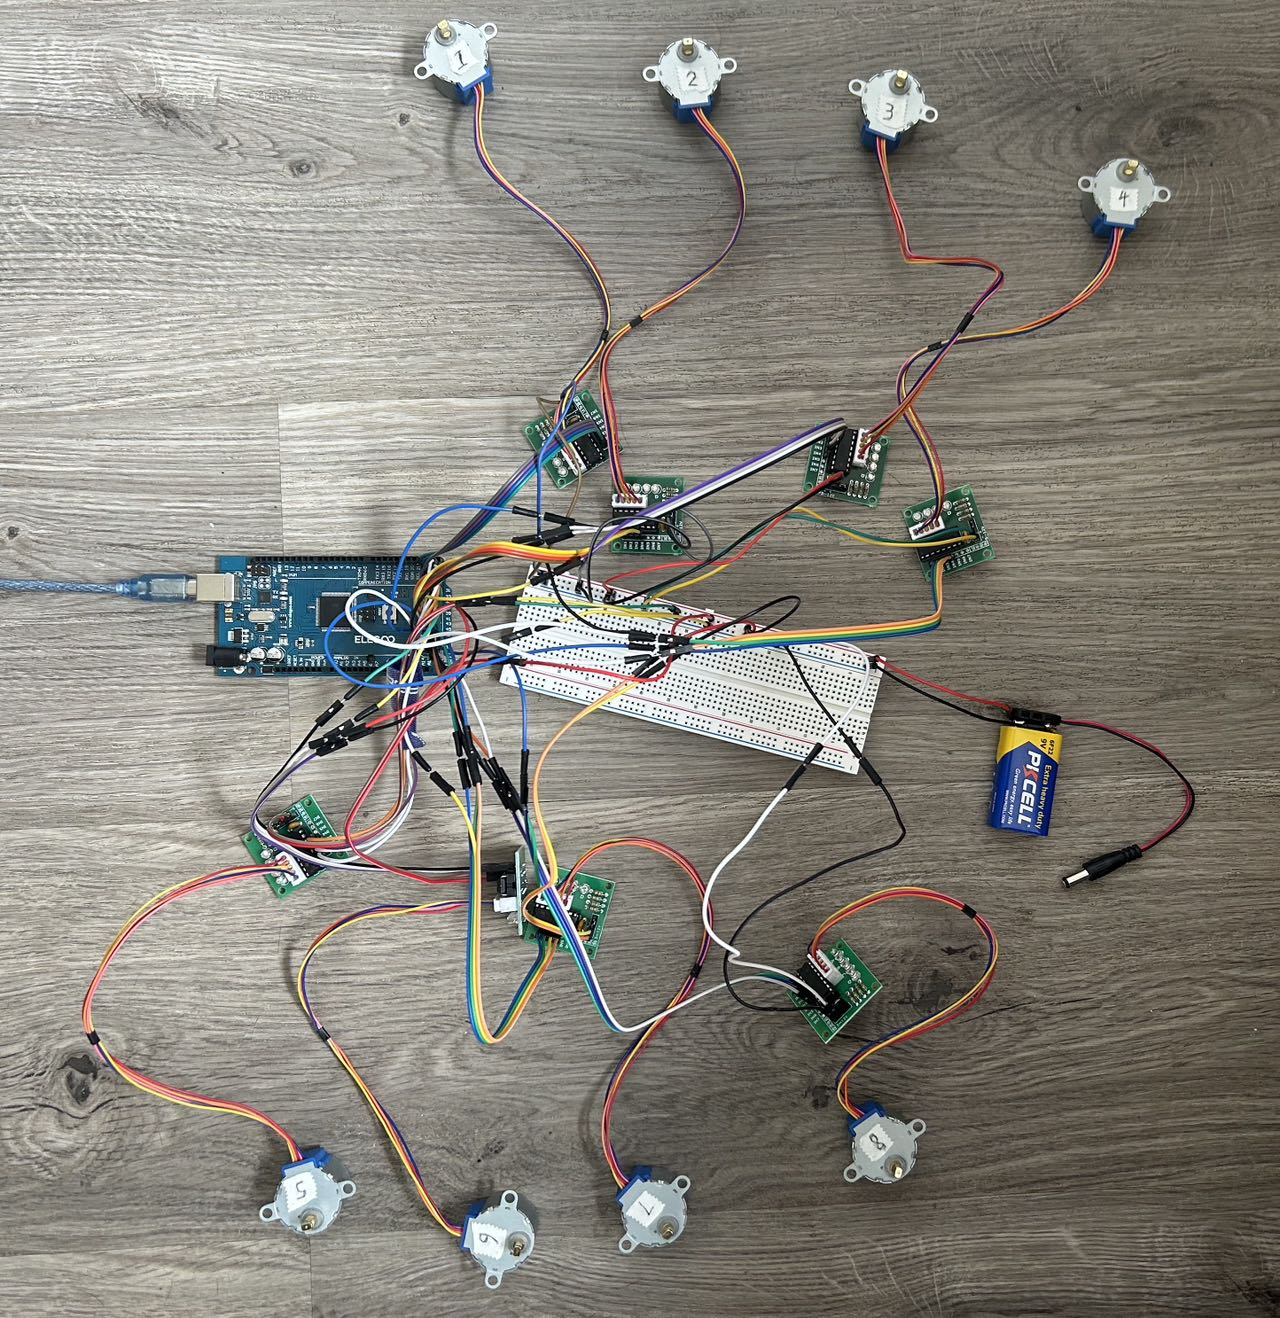
\includegraphics[width=0.9\textwidth]{Image/Result/circuit_connection.jpg} 
    \caption[The circuit connection of Arduino and stepper motors]
    {\centering \textbf{The circuit connection of Arduino and stepper motors.}}
    \label{fig:circuit_connection}
\end{figure}
\vspace{-5mm}
\noindent Users are required to sequentially input eight values of $\Delta S_1 \sim \Delta S_8$ to initiate 
the corresponding operation of the stepper motor. If the input is less than eight, the control system will 
not be executed. \\
According to Figure \ref{fig:arduino_code_display_1} in Appendix \ref{append:code_display}, the change volume 
of cables are input into the Arduino program for execution, with the input data series being $\boldsymbol{\Delta S}$ 
= [0, 0, -8, 8, -15, 15, 65, -65] (mm). The value of $\Delta S_i$ is always in pairs, e.g, two cables controlling 
the same unit should always have the opposite $\Delta S_i$ value, this is decided by the working principle of the 
manipulator. After conversion, the corresponding $Step_1 \sim Step_8$ is [0, 0, -521, 521, -978, 978, 4237, -4237] 
(steps), where the “-” sign represents counterclockwise steps. Afterwards, the stepping can be finished in certain 
time. The function \emph{Serial.print(motor.currentPosition())} can be utilized to check the steps of motors.\\
According to Figure \ref{fig:arduino_code_display_2} in Appendix \ref{append:code_display}, result of first testing 
is demonstrated, with all the motors are working appropriately. In this programme, all floating-point precision 
is taken to the $10^{-4}$ millimeter while the result printed on the monitor is $10^{-2}$ millimeter, 
which means that the accuracy of the result is acceptable.\\
Then, reset the motors, the motors went back to initial condition, which is $Step_1 \sim Step_8=0$. Repeat the 
motor stepping process, but this time, the motors are starting from a previous location from
$\boldsymbol{\Delta S_{now}}$ = [0, 0, -8, 8, -15, 15, 65, -65] (mm) to $\boldsymbol{\Delta S_{next}}$ = 
[33, -33, 16, -16, 0, 0, 10, -10] (mm). The difference $\boldsymbol{\Delta S_{diff}}$ = 
[33, -33, 24, -24, 15, -15, -55, 55] (mm), while the steps for motors are 
[2151, -2151, 1565, -1565, 978, -978, -3585, 3585] (steps). The result can be verified by checking how many 
revolutions each motor rotated in Figure \ref{fig:arduino_code_display_3} in Appendix \ref{append:code_display}.
The results are aligned with the calculation. Hence, the actuation control system runs correctly.
The Arduino programme is updated in GitHub repository in 
\href{https://github.com/yezehao/Compact-Continuum-Manipulator-Platform/tree/main/Arduino-Simulation}
{Arduino Simulation}. \\
Overall, the method of using Arduino to control the stepper motor and drive the manipulator is a feasible solution. 
Although the initial idea of using simulation software failed to yield satisfying results, the testing outcomes with 
real components solved this problem.\\
Additionally, from the perspective of test results, it can be observed that the precision of the stepper motors are 
very high, which is a great advantage for an open-loop (no feedback) system as it minimizes errors to the greatest 
extent. In the 28YBJ-48 motor parameter settings, full stepping configuration implies that the motor is divided into 
2048 steps per revolution. For a rotor driving a cable with a circumference of 31.416 mm, this means a resolution of 
0.01534 mm per step, which is enough to provide the accuracy required.\\
However, at the same time, there are some limitations to consider in this aspect. The most apparent limitation is that 
when cables wrap around the rotor, it effectively increases the diameter of the rotor, leading to some errors. For a 
cable with a total length of 68 mm, it can wrap around the rotor twice. Assuming the cable has a thickness of 1 mm, this 
would introduce a maximum error of approximately $ 31.416 / (31.416 + 2) = 0.05 $. Although in practice, it is unlikely 
that two layers of cable would perfectly stack on top of each other, this should be considered, because it's a factor 
that will cause errors. To solve this, an equation relating the length change of cables and the change in diameters 
should be deduced and applied in the program to minimize the potential error, but due to limited time, this part was 
not finished.\\
Furthermore, in this programme, only a rough setting for the step speed of the motors has been set. However, for 
achieving synchronization in starting/ending movement of each unit of the manipulator, more precise mathematical 
derivations for the speed of motors are required. In the following development process, it would be helpful to 
associate the speed of stepper motors with the distance to the target position, thereby dynamically setting a 
speed value for each motor to accomplish this synchronization. \\
Ultimately, the input parameters of the control system are $\boldsymbol{\Delta S}$, which consist of eight indices. 
It is inconvenient for users to input a series of indices. The Arduino programme can be optimized to take the 
angles $\boldsymbol{\theta}$ as input parameters, which only require the users to input four parameters. The Python 
version programme is uploaded in the GitHub and ready to be converted into Arduino programme.
\subsubsection{Information Acquisition and Display}
In the design of the sensing and control section, the following functionalities have been implemented. 
\begin{itemize}
    \item Keyboard Input Control for Stepper Motor \\
    The system allows users to input commands via an upper computer keyboard to drive the stepper motor by specifying 
    the number of steps. The motor parameters are displayed on an LCD screen.
    \item MPU6050 Sensor for End-Effector Orientation \\
    The MPU6050 sensor collects the orientation angles of the manipulator’s end effector. The real-time data is displayed 
    on an OLED screen to assist users. The accuracy is controlled within 0.1°, meeting precision requirements. However, 
    prolonged sensor operation leads to increased internal chip temperature, resulting in noticeable noise and yaw zero-point 
    drift issues.
    \item HC-SR04 Ultrasonic Sensor for Distance Measurement \\
    The HC-SR04 ultrasonic sensor measures the distance from the manipulator’s end effector to the target object in 
    the polar coordinate system. The collected data is updated in real-time on the OLED screen to aid user operations. 
    The accuracy is effectively controlled within 3 mm, meeting precision requirements.
\end{itemize}
Due to the lack of a proper spatial coordinate detection system for the manipulator’s end effector, a closed-loop system has not 
been established in this project. The primary improvement task is to construct a closed-loop system, with the core technology 
being the determination of the end effector’s three-dimensional coordinates. Feasible solutions include:
\begin{itemize}
    \item Integration of Acceleration Data from MPU6050 \\
    The MPU6050 sensor detects acceleration along three axes. Integrating acceleration twice over time theoretically yields 
    displacement along these axes, which can further be used to derive spatial position coordinates. However, this approach 
    has limitations. Despite compensating for errors and drift, the results from double integration will rapidly accumulate 
    over time. Thus, relying solely on MPU6050 cannot provide accurate coordinate information for precise feedback in a 
    closed-loop system.
    \item Adding a Two-Degree-of-Freedom Gimbal at the End-Effector \\
    By attaching a gimbal with two degrees of freedom to the end-effector, the ultrasonic sensor can rotate vertically to face 
    three mutually perpendicular walls in the operating environment. The gimbal’s motor angles will be derived based on the 
    MPU6050’s orientation angles, ensuring that the ultrasonic sensor measures distances along the coordinate axes. However, 
    this approach assumes a workspace shaped like a rectangular prism with at least three perpendicular solid walls.
    \item Visual Processing Using Computer Vision \\
    Employing visual processing techniques, such as using cameras to track the sensor’s end effector, can derive distances 
    and further calculate coordinates based on phase focusing algorithms.
\end{itemize}
Among the three methods, the second approach has relatively low costs and minimal implementation difficulty. Once the 
end effector’s coordinates are obtained, combining them with the MPU6050’s orientation data allows for closed-loop control 
feedback. Additionally, considering that the MPU6050 performs best in low-temperature environments, measures such as 
chip cooling are necessary.

% change to new page
\newpage % Result and Discussion
%%%%% Conclusion %%%%%
\section{Conclusion} 
The project provides an introduction to the background and justifies the selection of a  fishbone continuum manipulator. 
It demonstrated simulations based on the specified objectives, with the methodology encompassing structural modeling, 
kinematic derivation, and control system development.

In this report, structural modeling was conducted using Ansys for strength and strain analysis. The conclusion drawn was that 
rubber, serving as the backbone structure, exhibited sufficient strength, and the motor torque was adequate to provide the 
corresponding tension in the cables. However, it is important to note that fatigue loss has not been taken into consideration.

From the perspective of kinematics, the corresponding workspace was determined through forward kinematics. However, a limitation 
was observed in that a strong correlation exists between the majority of positions and orientations. On the other hand, inverse 
kinematics accurately reproduced the posture but existing some degree of error. A proposed method was introduced as a potential 
solution to address this issue.

The control system was implemented to manage functions such as motor control. Simultaneously, a set of sensor systems has 
been deployed to prepare for the upgrade to a closed-loop system.

In conclusion, this project exhibited a high level of completion and relative comprehensiveness. All content, including this 
report, has been uploaded to GitHub, accompanied by corresponding README files and code comments to guide users in executing 
the programmes. The \href{https://github.com/yezehao/Compact-Continuum-Manipulator-Platform}{GitHub Repository} can be accessed 
through https://github.com/yezehao/Compact-Continuum-Manipulator-Platform .



% change to new page
\newpage % Conclusion



\printbibliography[title = {References}]
\addcontentsline{toc}{chapter}{References}
\end{document}
%------------------------------------------The Document Ends here--------------------------------------------